\documentclass[twoside,11pt]{article}

% Any additional packages needed should be included after jmlr2e.
% Note that jmlr2e.sty includes epsfig, amssymb, natbib and graphicx,
% and defines many common macros, such as 'proof' and 'example'.
%
% It also sets the bibliographystyle to plainnat; for more information on
% natbib citation styles, see the natbib documentation, a copy of which
% is archived at http://www.jmlr.org/format/natbib.pdf

\usepackage{jmlr2e}

\usepackage{algpseudocode}
\usepackage{algorithm}
\usepackage{amsmath}
\usepackage{amssymb}
\usepackage{float}
\usepackage{graphicx}
\usepackage{multirow}
\usepackage[caption = false]{subfig}

% Definitions of handy macros can go here

\newcommand{\dataset}{{\cal D}}
\newcommand{\fracpartial}[2]{\frac{\partial #1}{\partial  #2}}

% \newtheorem{proposition}{Proposition}

% Heading arguments are {volume}{year}{pages}{submitted}{published}{author-full-names}

\jmlrheading{1}{2016}{1-48}{4/00}{10/00}{Theodore Papamarkou and Eric Ford}

% Short headings should be running head and authors last names

\ShortHeadings{Manifold Langevin Monte Carlo with Partial Metric Updates}{Papamarkou and Ford}
\firstpageno{1}

\begin{document}

\title{Manifold Langevin Monte Carlo with Partial Metric Updates}

\author{\name Theodore Papamarkou
	     \email theodore.papamarkou@glasgow.ac.uk\\
       \addr School of Mathematics and Statistics\\
       University of Glasgow, UK
       \AND
       \name Eric Ford
       \email ebf11@psu.edu\\
       \addr Center for Astrostatistics\\
       Pennsylvania State University, USA
}

\editor{Leslie Pack Kaelbling}

\maketitle

\begin{abstract}%   <- trailing '%' for backward compatibility of .sty file
Manifold Markov chain Monte Carlo algorithms have been introduced to sample more effectively from challenging target 
densities exhibiting multiple modes or strong correlations. Such algorithms exploit the local geometry of the parameter 
space, thus simulating chains with high convergence rate. However, acquiring local geometric information increases 
computational complexity to the extent that sampling from high-dimensional targets becomes inefficient.
This paper proposes a manifold Langevin Monte Carlo framework aimed at maintaining a feasible amount of geometric 
computation. The suggested strategy regulates the frequency of manifold-based updates via a schedule, hence it controls the 
trade-off between effective sample size and computational cost leading to improved computational efficiency. An 
exponentially decaying schedule is put forward that enables more frequent updates of geometric information in early 
transient phases of the chain, while saving computational time in late stationary phases. Alternatively, a modulo schedule 
is introduced to allow sparse yet recurring geometric updates throughout the sampling course, acting as a correction 
mechanism for adaptive proposals that learn the covariance structure of the parameter space. The average complexity can be 
manually set for either of these two schedules depending on the need for geometric exploitation posed by the underlying 
model.
\end{abstract}

\begin{keywords}
  Bayesian inference,
  High-dimensional data analysis,
  Markov chain Monte Carlo,
  Langevin Monte Carlo	
\end{keywords}

\section{Introduction}

The birth of geometric-based Markov chain Monte Carlo (MCMC) dates back to the landmark paper of \cite{dua_ken_pen__hyb},
which introduced Hamiltonian Monte Carlo (HMC) to unite MCMC with molecular dynamics.
\cite{dua_ken_pen__hyb} applied HMC in lattice field theory simulations of quantum chromodynamics.
Statistical applications of HMC began with its use in neural network models by \cite{nea__bay}.

In the meanwhile, the Metropolis-adjusted Langevin algorithm (MALA) was proposed by \cite{rob_ros__opt} to harness Langevin 
dynamics for proposing new states in MCMC simulations. Both HMC and MALA evaluate the gradient of the target density, so 
they utilize local geometric flow.

The seminal work of \cite{gir_cal__rie} raised awareness of the differential geometric foundations of MCMC. Given a vector 
of parameters $\boldsymbol{\theta}\in\mathbb{R}^{n_\theta}$, \cite{gir_cal__rie} defines a distance between two probability 
densities $p(\boldsymbol{\theta})$ and $p(\boldsymbol{\theta}+\delta\boldsymbol{\theta})$ as the quadratic form
$\delta\boldsymbol{\theta}^T G(\boldsymbol{\theta}) \delta\boldsymbol{\theta}$ for an arbitrary metric 
$G(\boldsymbol{\theta})$. Thus, the position-specific metric $G(\boldsymbol{\theta})$ induces a Riemann manifold in the 
space of parameterized probability density functions $\left\{p(\boldsymbol{\theta}):\boldsymbol{\theta}\right\}$.
In the context of MCMC, $G(\boldsymbol{\theta})$ depends on the current state $\boldsymbol{\theta}$ of the simulated Markov 
chain. \cite{gir_cal__rie} uses $G(\boldsymbol{\theta})$ to define transition kernels that explore the parameter space
$\left\{\boldsymbol{\theta}:\boldsymbol{\theta}\in\mathbb{R}^{n_\theta}\right\}$ effectively, thereby introducing Riemann 
manifold Langevin and Hamiltonian Monte Carlo methods.

The differential geometric basis of MCMC has been further researched since the appearance of \cite{gir_cal__rie}. For 
instance, \cite{byr_gir__geo} developed proposal mechanisms by following geodesic flows over the embedded manifolds of 
support for the target distribution. \cite{lan_sta_sha__mar} replaced the auxiliary momentum variable appearing in Riemann 
manifold Hamiltonian Monte Carlo (RMHMC) by velocity to develop a Markov chain Monte Carlo algorithm using Lagrangian 
dynamics. \cite{lan_str_sha__wor} defined the so-called wormhole metric, for which distance between modes is shortened, in 
order to facilitate transitions between modes of multimodal target densities.

Computing the geometric entities of differential geometric MCMC methods creates a performance bottleneck that restricts the 
applicability of the involved methods. For example, manifold Monte Carlo methods require to calculate the metric tensor
$G(\boldsymbol{\theta})$ of choice. Typically, $G(\boldsymbol{\theta})$ is set to be the observed Fisher information matrix,
which equals the negative Hessian of the log-target density at a specific point $\boldsymbol{\theta}$.
Consequently, the complexity of manifold MCMC algorithms is dominated by Hessian-related computations, including inversion of
the Hessian, so it becomes at best of order $\mathcal{O}(n_\theta^3)$.

In spite of being of order $\mathcal{O}(n_\theta^3)$ too, the simplified manifold Metropolis-adjusted Langevin algorithm 
(SMMALA) introduced by \cite{gir_cal__rie} is faster than MMALA and RMHMC in lower-dimensional parameter spaces. The 
relatively faster speed of SMMALA over MMALA and RMHMC is explained by lower order terms and constant factors appearing in 
big-oh notation, which are ordinarily omitted but affect runtime in the case of smaller $n_\theta$. For this reason, the 
simplified manifold Metropolis adjusted Langevin algorithm (SMMALA) has been employed in conjunction with population MCMC 
for the Bayesian analysis of mechanistic models based on systems of non-linear differential equations, see 
\cite{cal_gir__sta} and \cite{sch_pap__ews}. Despite the capacity of SMMALA to exploit local geometric information so as to 
cope with non-linear correlations and modest increase in the dimensionality of the parameter space, in other cases its 
computational complexity can render the performance inferior to other algorithms such as the Metropolis-adjusted Langevin 
algorithm (MALA) or adaptive MCMC, see \cite{cal_eps_sil__bay}.

Various attempts have been made to ameliorate the computational implications of geometric Monte Carlo methods. Along these 
lines, \cite{lan_tha_chr__emu} used Gaussian processes to emulate the Hessian matrix and Christoffel symbols associated with 
the observed Fisher information $G(\boldsymbol{\theta})$. \cite{sim_bad_cem__sto} developed a stochastic quasi-Newton 
Langevin MCMC algorithm which takes into account the local geometry, while approximating the inverse Hessian by using a 
limited history of samples and their gradients. Alternatively, \cite{per__prox} used convex analysis and proximal techniques 
instead of differential calculus in order to construct a Langevin Monte Carlo method for high-dimensional target 
distributions that are log-concave and possibly not continuously differentiable.

This paper develops a Monte Carlo method that capitalizes on the sampling effectiveness of SMMALA and at the same time 
breaks the computational barrier of $\mathcal{O}(n_\theta^3)$. The proposed method permits to adjust the schedule of metric
updates. Moreover, it is simple to implement and it performs exact metric evaluations, avoiding emulation or other 
approximations of the Hessian of the log-target density.

\section{Background}

The role of this section is to provide a brief overview of Langevin Monte Carlo and to stage a unified notation, which will
be used for introducing the method contributed by this paper.

From a statistical perspective, Langevin Monte Carlo is a special case of Metropolis-Hastings with a normal proposal
distribution
\begin{equation}
\label{langevin_proposal}
q(\boldsymbol{\theta}^{\star}|\boldsymbol{\theta}) =
\mathcal{N}(\boldsymbol{\theta}^{\star}|\boldsymbol{\mu}(\boldsymbol{\theta}, G, \epsilon), \Sigma(G, \epsilon)),
\end{equation}
where $\boldsymbol{\theta}^{\star}$ and $\boldsymbol{\theta}$ denote the respective proposed and current state, $G$ is a
positive definite matrix of size $n_{\theta} \times n_{\theta}$ and $\epsilon$ refers to a tuning parameter known as the
integration stepsize. The location $\boldsymbol{\mu}(\boldsymbol{\theta}, G, \epsilon)$ is a function of 
$\boldsymbol{\theta}$, $G$ and $\epsilon$, whereas the covariance $\Sigma(G, \epsilon)$ of the proposal density depends on 
$G$ and $\epsilon$. Both $\boldsymbol{\mu}(\boldsymbol{\theta}, G, \epsilon)$ and $\Sigma(G, \epsilon)$ are defined so that 
the proposed states admit a Langevin diffusion approximated by a first-order Euler discretization. In other words, the 
Langevin diffusion has a stationary distribution $p(\boldsymbol{\theta})$, so a Markov chain simulated from the 
Metropolis-Hastings scheme outlined by proposal \eqref{langevin_proposal} will converge to the target 
$p(\boldsymbol{\theta})$. The Metropolis-Hastings acceptance probability is to its standard form
\begin{equation}
\label{langevin_acceptance}
a(\boldsymbol{\theta},\boldsymbol{\theta}^{\star}) =
\min\left\{
\frac{p(\boldsymbol{\theta}^{\star})q(\boldsymbol{\theta}|\boldsymbol{\theta}^{\star})}
{p(\boldsymbol{\theta})q(\boldsymbol{\theta}^{\star}|\boldsymbol{\theta})}
, 1
\right\}.
\end{equation}

The integration stepsize $\epsilon$ is associated with the first order Euler discretization and its value affects the
state space exploration. If $\epsilon$ is selected to be relatively large, some of the proposed candidates will be far from 
the current state, and will therefore have a low probability of acceptance, so the generated chain will have low acceptance 
rate. Reducing $\epsilon$ will increase the acceptance rate, but the chain will take longer to traverse the state space.

In a Bayesian setting, the target is a possibly unnormalized posterior distribution $p(\boldsymbol{\theta}|\mathbf{y})$,
where $\mathbf{y}$ denotes the available data. Replacing $p(\boldsymbol{\theta})$ by $p(\boldsymbol{\theta}|\mathbf{y})$ in
\eqref{langevin_acceptance} makes Langevin Monte Carlo applicable in Bayesian problems.

To fully specify a Langevin Monte Carlo algorithm, the location $\boldsymbol{\mu}(\boldsymbol{\theta}, G, \epsilon)$ and 
covariance $\Sigma(G, \epsilon)$ of normal proposal \eqref{langevin_proposal} need to be defined. In what follows, 
variations of geometric Langevin Monte Carlo methods are distinguished by their respective proposal location and covariance.

\subsection{Metropolis-Adjusted Langevin Algorithm}
\label{mala_section}

If $G$ is kept constant, that is if $G$ is a not a function of the current state $\boldsymbol{\theta}$, then the
Metropolis-adjusted Langevin algorithm (MALA) arises as
\begin{eqnarray}
\label{mala_location}
\boldsymbol{\mu}(\boldsymbol{\theta}, G, \epsilon) = 
\boldsymbol{\theta}+\frac{\epsilon^2}{2}G^{-1}\nabla_{\theta}\log{p(\boldsymbol{\theta})},\\
\label{mala_covariance}
\Sigma(G, \epsilon) = \epsilon^2 G^{-1}.
\end{eqnarray}
$G$ is known as the precondition matrix, see \cite{rob_stra__lan}. It is typically set to be the identity matrix $G=I$, in
which case MALA is defined in its conventional form
\begin{equation}
\label{mala_location_covariance_identity}
\boldsymbol{\mu}(\boldsymbol{\theta}, \epsilon) = 
\boldsymbol{\theta}+\frac{\epsilon^2}{2}\nabla_{\theta}\log{p(\boldsymbol{\theta})},~
\Sigma(\epsilon) = \epsilon^2 I.
\end{equation}

According to the theoretical analysis of \cite{rob_ros__opt}, the optimal scaling $\epsilon$ has been found to be the value 
of $\epsilon$ which yields a limiting acceptance rate of $57.4\%$ in high-dimensional parametric spaces 
(as $n_{\theta}\rightarrow\infty$).

\subsection{Manifold Langevin Monte Carlo Algorithms}
\label{smmala_section}

MALA uses the gradient flow $\nabla_{\theta}\log{p(\boldsymbol{\theta})}$ to make proposals effectively.
As explained by \cite{gir_cal__rie}, it is possible to incorporate further geometric structure in the form of a 
position-dependent metric $G(\boldsymbol{\theta})$.
This way, the Langevin diffusion is defined on a Riemann manifold endowed by the metric $G(\boldsymbol{\theta})$, and the
corresponding Levi-Civita connection specified by the Christoffel symbols of second-kind 
$\Gamma^{k}_{ij}(\boldsymbol{\theta})$. The resulting manifold Metropolis-adjusted Langevin algorithm (MMALA) draws 
candidate states from a normal proposal with location and covariance given by
\begin{eqnarray}
\label{mmala_location}
\boldsymbol{\mu}_{(k)}(\boldsymbol{\theta}, G(\boldsymbol{\theta}), \epsilon) =
\boldsymbol{\theta}+
\frac{\epsilon^2}{2}(G^{-1}(\boldsymbol{\theta})\nabla_{\theta}\log{p(\boldsymbol{\theta})})_{(k)}-
\epsilon^2\sum_{i,j=1}^{n_\theta}G^{-1}_{ij}(\boldsymbol{\theta})\Gamma^{k}_{ij}(\boldsymbol{\theta}),\\
\label{mmala_covariance}
\Sigma(G(\boldsymbol{\theta}), \epsilon) = \epsilon^2 G^{-1}(\boldsymbol{\theta}),
\end{eqnarray}
where $\boldsymbol{\mu}_{(k)}$ refers to the $k$-th coordinate of proposal location
$\boldsymbol{\mu}(\boldsymbol{\theta}, G(\boldsymbol{\theta}), \epsilon)$.

If a manfiold of constant curvature is assumed, then the Christoffel symbols vanish, so the proposal location of MMALA
simplifies to
\begin{equation}
\label{smmala_location}
\boldsymbol{\mu}(\boldsymbol{\theta}, G(\boldsymbol{\theta}), \epsilon) =
\boldsymbol{\theta}+
\frac{\epsilon^2}{2}G^{-1}(\boldsymbol{\theta})\nabla_{\theta}\log{p(\boldsymbol{\theta})}.
\end{equation}
The method associated with location \eqref{smmala_location} is known as simplified Metropolis-adjusted Langeving algorithm
(SMMALA). As seen from the location and covariance of their proposal mechanisms, MALA is a special case of SMMALA, which is 
in turn a special case of MMALA.

The optimal stepsize $\epsilon$ for MMALA and SMMALA is empirically suggested by \cite{gir_cal__rie} to be set so as to 
obtain an acceptance rate of around $70\%$; this choice has not been analyzed yet from a theoretical standpoint analogously 
to the choice of scaling for MALA by \cite{rob_ros__opt}.

\section{Partial Manifold Langevin Metric Updates}

\subsection{Motivation}
\label{Motivation}

To dissect the incurring computational cost of geometric MCMC methods, it suffices to consider their three common steps
that dominate computation. In brief, these three steps include sampling from the proposal, evaluating the proposal density,
and for some geometric schemes evaluating the derivatives of the metric tensor.

Ordinarily, the proposal used in Langevin Monte Carlo is set to be a multivariate normal distribution
$
q(\boldsymbol{\theta}^{\star}|\boldsymbol{\theta}) =
\mathcal{N}(\boldsymbol{\theta}^{\star}|
\boldsymbol{\mu}(\boldsymbol{\theta}, G, \epsilon), \epsilon^2 G^{-1}(\boldsymbol{\theta}))
$,
as seen in \eqref{langevin_proposal}, \eqref{mala_covariance} and \eqref{mmala_covariance}. To propose a state 
$\boldsymbol{\theta}^{\star}$, the proposal is typically simulated in the Cholesky approach by letting
\begin{equation}
\boldsymbol{\theta}^{\star} =
\boldsymbol{\mu}(\boldsymbol{\theta}, G, \epsilon)+
\epsilon \left(\sqrt{G^{-1}(\boldsymbol{\theta})}\right)^{'}\tau
\end{equation}
where $\sqrt{G^{-1}(\boldsymbol{\theta})}$ satisfies the Cholesky decomposition
$
\left(\sqrt{G^{-1}(\boldsymbol{\theta})}\right)^{'}\sqrt{G^{-1}(\boldsymbol{\theta})}=
G^{-1}(\boldsymbol{\theta})
$
and $\tau\sim\mathcal{N}(\mathbf{0}, I)$, \cite{chi_gre__und}.
So, sampling from the proposal has a complexity of $\mathcal{O}(2n_\theta^3)$, since it requires the inversion of metric 
$G(\boldsymbol{\theta})$ and the Cholesky decomposition of $G^{-1}(\boldsymbol{\theta})$, each of which are
$\mathcal{O}(n_\theta^3)$ operations. MALA, as opposed to SMMALA and MMALA, relies on a constant preconditioning matrix G,
therefore $G^{-1}$ and $\sqrt{G^{-1}}$ are evaluated once and cached at the beginning of the simulation avoiding the
$\mathcal{O}(n_\theta^3)$ cost.

To calculate the Metropolis-Hastings acceptance ratio \eqref{langevin_acceptance} appearing in SMMALA and MMALA,
it is required to evaluate the normal proposal twice. As it has become apparent, a proposal evaluation has a complexity of
$\mathcal{O}(n_\theta^3)$ due to the proposal covariance $\epsilon^2 G^{-1}(\boldsymbol{\theta})$ entailing the inversion of 
$G(\boldsymbol{\theta})$. Once again, MALA avoids the $\mathcal{O}(n_\theta^3)$ penalty at proposal evaluations as the
position-independent inverse $G^{-1}$ is initially computed and is then kept fixed.

MMALA and RMHMC, as introduced by \cite{gir_cal__rie}, additionally require to compute the Christoffel symbols 
$\Gamma^{k}_{ij}(\boldsymbol{\theta})$, which involve
the partial derivatives $\partial G(\boldsymbol{\theta})/\partial\theta_k,~k\in\left\{1,2,\dots,n_{\theta}\right\},$
of metric $G(\boldsymbol{\theta})$. If $G(\boldsymbol{\theta})$ is chosen to be the 
observed Fisher information matrix, $\partial G(\boldsymbol{\theta})/\partial\theta_k$ represent the partial derivatives of 
the negative Hessian, that is they are equal to minus the third-order partial derivatives of the log-target density 
$\log{p(\boldsymbol{\theta})}$, thereby the computation of $\partial G(\boldsymbol{\theta})/\partial\theta_k$ is an 
operation of order $\mathcal{O}(n_\theta^3)$. Since the Christoffel symbols vanish in the case of SMMALA, the cost of
$\mathcal{O}(n_\theta^3)$ for the computation of $\partial G(\boldsymbol{\theta})/\partial\theta_k$ is not inflicted on
SMMALA.

To sum up, MMALA necessitates computing the two matrix inverses $G^{-1}(\boldsymbol{\theta})$ and 
$G^{-1}(\boldsymbol{\theta}^{\star})$ in order to evaluate the proposals involved in the acceptance probability 
\eqref{langevin_acceptance}, one Cholesky decomposition $\sqrt{G^{-1}(\boldsymbol{\theta})}$ to sample from the proposal, 
and the third-order derivatives $\partial G(\boldsymbol{\theta})/\partial\theta_k$ of $G(\boldsymbol{\theta})$
for learning the curvature of the associated manifold. Hence, MMALA has a complexity of $\mathcal{O}(4n_\theta^3)$. SMMALA
poses the same computational requirements apart from setting $\partial G(\boldsymbol{\theta})/\partial\theta_k$ to zero, so 
the complexity of SMMALA becomes $\mathcal{O}(3n_\theta^3)$.

Owing to the works of \cite{dav_sto__imp}, \cite{wil__brea} and \cite{leg__pow},
optimized versions of the Coppersmith-Winograd algorithm allow to perform matrix multiplication and therefore matrix 
inversion in $\mathcal{O}(n_\theta^{2.373})$ time. Consequently, optimized implementations of MMALA and SMMALA can run in
$\mathcal{O}(2n_\theta^3+2n_\theta^{2.373})$ and $\mathcal{O}(n_\theta^3+2n_\theta^{2.373})$ time, respectively.

A detailed account of the time complexity of SMMALA has been given to highlight the main sources of computational load
involved in geometric updates. In what follows, scaling factors and constants will be suppressed in big-$\mathcal{O}$ 
notation following common practice.

Since the preconditioning matrix $G$, its inverse $G^{-1}$ and the Cholesky decomposition $\sqrt{G^{-1}}$ are cached upon 
initialization for MALA, the quadratic form
$
(\boldsymbol{\theta}^{\star}-\boldsymbol{\theta}^{\star})'
G^{-1}
(\boldsymbol{\theta}^{\star}-\boldsymbol{\theta}^{\star})
$
in the normal proposal density dictates a time complexity of $\mathcal{O}(n_{\theta}^2)$ for MALA. If $G$ is set to be the 
identity matrix, then
$
(\boldsymbol{\theta}^{\star}-\boldsymbol{\theta}^{\star})'
G^{-1}
(\boldsymbol{\theta}^{\star}-\boldsymbol{\theta}^{\star})
$
reduces to the inner product
$
\langle\boldsymbol{\theta}^{\star}-\boldsymbol{\theta}^{\star},
\boldsymbol{\theta}^{\star}-\boldsymbol{\theta}^{\star}\rangle
$. This inner product and the gradient $\nabla_{\theta}\log{p(\boldsymbol{\theta})}$  of the log-target have a complexity of 
$\mathcal{O}(n_{\theta})$ each. So, if $G=I$, the complexity of MALA is of order $\mathcal{O}(n_{\theta})$.

An implicit assumption made for all the complexity bounds of this section is that the log-target evaluations do not
exceed the complexity of the associated samplers. Of course there are models for which such assumption is not plausible.
For instance, if the underlying model consists of a system of non-linear ordinary differential equations (ODEs) and each 
log-target calculation requires solving the ODE system numerically, then the log-target evaluations might dominate the
cost of the MCMC simulation depending on the size of the parameter and state space and on the complexity of the numerical 
ODE solver.

Combining the best of two worlds, an effective and efficient MCMC algorithm would exploit geometric information in time as 
close as possible to the linear time of MALA. One potential approach towards this end would be to approximate the expensive 
components of geometric computation, such as $G^{-1}(\boldsymbol{\theta})$ and $\sqrt{G^{-1}(\boldsymbol{\theta})}$, in the 
spirit of \cite{sim_bad_cem__sto}. An alternative route, taken by the present paper, is to design a hybrid sampling method 
that switches between expensive geometrically-informed and cheaper non-geometric proposal mechanisms. The latter idea is
motivated by the objective to exploit exact geometric updates whenever these occur, therefore not rendering each Monte Carlo 
iteration approximate.

\subsection{Partial Manifold Langevin Metric Updates in MALA}

Sections \ref{mala_section} and \ref{smmala_section} provide a unified formulation of MALA and SMMALA. More specifically, 
both samplers constitute variations of a Metropolis-Hastings algorithm with a normal proposal given by 
\eqref{langevin_proposal} and acceptance probability defined by \eqref{langevin_acceptance}. The MALA and SMMALA normal 
proposals differ in their locations and covariances, which are specified by \eqref{mala_location}-\eqref{mala_covariance} 
and \eqref{smmala_location}-\eqref{mmala_covariance} respectively. From an algorithmic perspective, the natural way to 
switch between MALA and SMMALA updates is to variably rely on the locations and covariances of their associated 
candidate-generating kernels.

Both MALA and SMMALA learn from the local geometry of the underlying manifold. MALA resorts to gradient flow computations, 
while SMMALA further enriches its geometric information by incorporating the position-specific metric 
$G(\boldsymbol{\theta})$ to the updating mechanism. So, strictly speaking, a hybrid algorithm that switches between MALA and 
SMMALA proposals combines two geometric MCMC methods with varying levels of geometric information and of computational cost. 
To keep the resulting complexity as low as possible, the bulk of transitions should be driven by MALA, allowing intervening 
SMMALA updates to occur just frequently enough to boost sampling effectiveness.

A first question is how to pick from the MALA and SMMALA proposals at each MCMC iteration. One possibility is to make a
random choice via a Bernoulli trial. At the $i$-th iteration, draw a sample $b(i)\sim \mbox{Bernoulli}(p(i))$ with
probability $p(i)$ of taking a SMMALA step. If $b(i)=0$ then propose a new state $\boldsymbol{\theta}^{\star}$ sampled from
the MALA proposal, whereas if $b(i)=1$ then propose $\boldsymbol{\theta}^{\star}$ drawn from the SMMALA proposal.

Secondly, there needs to be a way of selecting the probabilities $p(i)$ as a function of the current iteration
$i\in\left\{1,2,\cdots,n_m\right\}$, where $n_m$ is the total number of MCMC steps. In other words, a schedule is needed for
the probabilities $p(i)$ of choosing between MALA and SMMALA updates. One possible choice of $p(i)$ is an exponentially 
decaying schedule
\begin{equation}
\label{exp_schedule_a}
p(i)=\exp{(-a(i-1)/n_m)},
\end{equation}
where $a$ denotes a constant tuning factor that determines the decay rate of $p(i)$.
Schedule \eqref{exp_schedule_a} makes SMMALA updates more probable in early transient iterations of the chain, while it 
makes MALA updates increasingly more likely in late stationary iterations. Hence, as the chain converges, less geometric 
information is acquired to reduce the computational load. Figure \ref{fig:exp_schedule_a} displays the schedule of Bernoulli 
probabilities for varying decaying rates.

\begin{figure}[t]
	\centering
	\subfloat[$b=0$]{
		\label{fig:exp_schedule_a}
		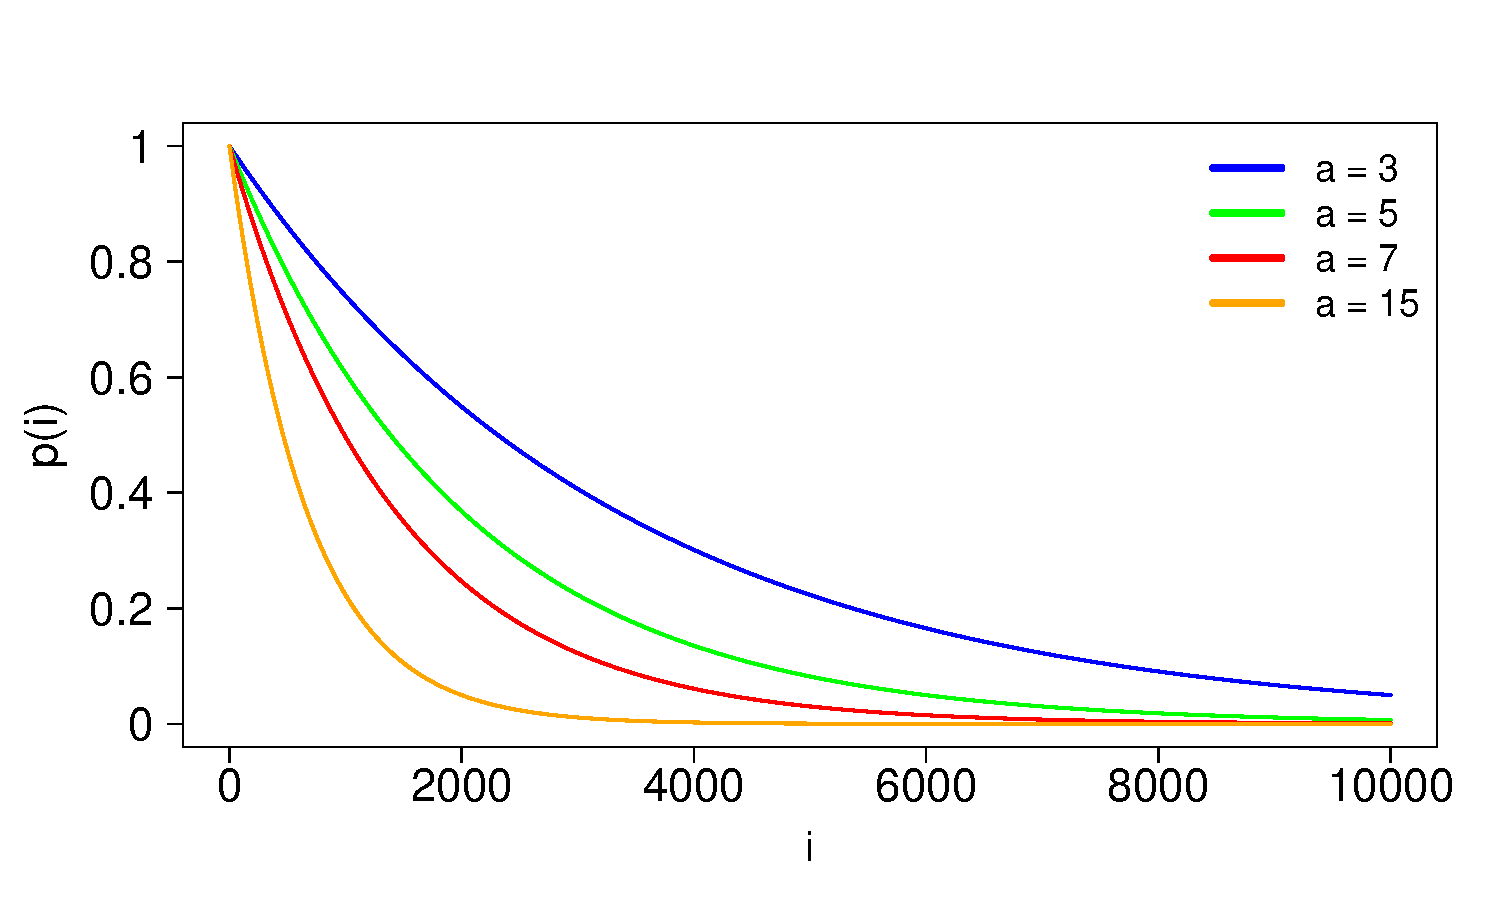
\includegraphics[width=2.3in]{exp_schedule_a.pdf}
	}
	\subfloat[$b=0.1$]{
	  \label{fig:exp_schedule_a_b}
		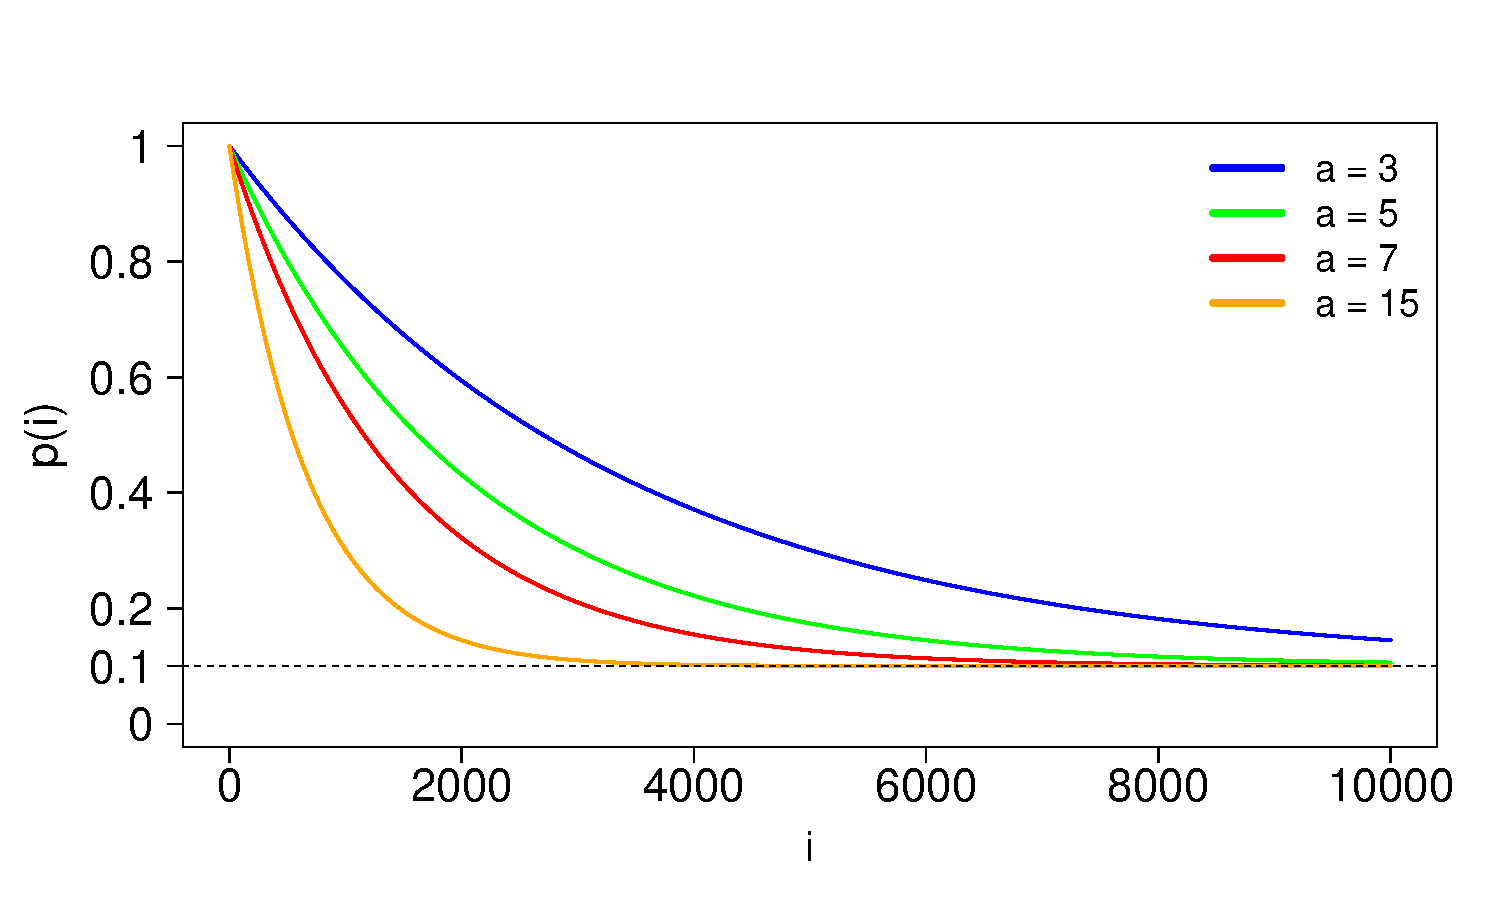
\includegraphics[width=2.3in]{exp_schedule_a_b.pdf}
	} \\
	\caption{Exponentially decaying schedule of probabilities $p(i)$ of making SMMALA proposals as a function of
	$i$-th MCMC iteration. The tuning factor $b$ sets the asymptotic probability of selecting the SMMALA proposal mechanism
	over its MALA counterpart. On the other hand, the tuning factor $a$ determines the rate of decay of $p(i)$ with larger 
	$a$ corresponding to more rapid decay.}
	\label{fig:exp_schedule}
\end{figure}

Subject to the model under consideration, it might be desirable to maintain a certain probability $b$ of making SMMALA 
proposals in late MCMC iterations instead of eliminating this probability. Schedule \eqref{exp_schedule_a} can be modified as
\begin{equation}
\label{exp_schedule_a_b}
p(i)=(1-b)\exp{(-a(i-1)/n_m)}+b,
\end{equation}
where the additional tuning factor $b$ sets the asymptotic probability of using the SMMALA proposal mechanism in late MCMC
iterations. Obviously \eqref{exp_schedule_a} arises as a special case of \eqref{exp_schedule_a_b} by setting $b=0$ in the 
latter equation. Figure \ref{fig:exp_schedule_a_b} visualizes schedule \eqref{exp_schedule_a_b} for varying decaying rates 
and for $b=0.1$, which corresponds to a $10\%$ probability of picking SMMALA proposals as the simulation progresses towards 
its end.

A third and last question to be addressed in order to fully construct the hybrid sampler is how to set the preconditioning 
matrix for MALA proposals. One way to proceed is to use the most recent metric $G(\boldsymbol{\theta}^0)$ computed at the 
latest state $\boldsymbol{\theta}^0$ obtained via a SMMALA update. This is where the computational gain comes from, since 
$G(\boldsymbol{\theta}^0)$, $G^{-1}(\boldsymbol{\theta}^0)$ and $\sqrt{G^{-1}(\boldsymbol{\theta}^0)}$ are cached and reused 
for the intervening MALA steps between successive SMMALA updates. An alternative option is to utlilize an identity 
preconditioning matrix $G=I$ corresponding to MALA proposal densities of the form
$\mathcal{N}(\boldsymbol{\theta}+\frac{\epsilon^2}{2}\nabla_{\theta}\log{p(\boldsymbol{\theta})}, \epsilon^2 I)$,
thus adhering to the most commonly used version of MALA.

The resulting algorithm is abbreviated as ALSMMALA. The AL prefix implies that the bulk of states are drawn from a MALA 
proposal mechanism and the SMMALA suffix indicates that the local geometry is exploited via more expensive SMMALA updates.
Algorithm \ref{alsmmala} provides pseudocode to summarize ALSMMALA for some schedule $p(i)$.

\begin{algorithm}[t]
	\caption{ALSMMALA}
	\label{alsmmala}
	\begin{algorithmic}
		\State $\boldsymbol{\theta}^{\circ}=\boldsymbol{\theta}$\\
		
		\For{$k = 1$ to $n_m$} % \Comment{$n$: number of iterations}
		\State Sample $b \sim \mbox{Bernoulli}(p(i))$\\
		
		\State Sample $u\sim\mathcal{U}(0, 1)$\\
		
		\If {$b = 0$} \Comment{Use MALA proposal}
		\State Sample 
		$\boldsymbol{\theta^{*}}
		\sim\mathcal{N}(\boldsymbol{\mu}(\boldsymbol{\theta}, G(\boldsymbol{\theta}^{\circ}), \epsilon),
		\epsilon^2 G^{-1}(\boldsymbol{\theta}^{\circ}))
		$\\
		
		\If
		{
			$u<\dfrac{
				p(\boldsymbol{\theta}^{*})
				\mathcal{N}(\boldsymbol{\theta}|
					\boldsymbol{\mu}(\boldsymbol{\theta}^{*},
					G(\boldsymbol{\theta}^{\circ}),
					\epsilon),
					\epsilon^2 G^{-1}(\boldsymbol{\theta}^{\circ}))
			}
			{
				p(\boldsymbol{\theta})
				\mathcal{N}(\boldsymbol{\theta}^{*}|
					\boldsymbol{\mu}(\boldsymbol{\theta},
					G(\boldsymbol{\theta}^{\circ}),
					\epsilon),
					\epsilon^2 G^{-1}(\boldsymbol{\theta}^{\circ}))
			}$
		}
		
		\State $\boldsymbol{\theta}=\boldsymbol{\theta}^{*}$
		\EndIf
		\ElsIf {$b=1$} \Comment{Use SMMALA proposal}
		\State Sample 
		$\boldsymbol{\theta^{*}}
		\sim\mathcal{N}(\boldsymbol{\mu}(\boldsymbol{\theta}, G(\boldsymbol{\theta}), \epsilon),
		\epsilon^2 G^{-1}(\boldsymbol{\theta}))
		$\\
		
		\If
		{
			$u<\dfrac{
				p(\boldsymbol{\theta}^{*})
				\mathcal{N}(\boldsymbol{\theta}|
					\boldsymbol{\mu}(\boldsymbol{\theta}^{*},
					G(\boldsymbol{\theta}^{*}),
					\epsilon),
					\epsilon^2 G^{-1}(\boldsymbol{\theta}^{*}))
			}
			{
				p(\boldsymbol{\theta})
				\mathcal{N}(\boldsymbol{\theta}^{*}|
					\boldsymbol{\mu}(\boldsymbol{\theta},
					G(\boldsymbol{\theta}),
					\epsilon),
					\epsilon^2 G^{-1}(\boldsymbol{\theta}))
			}$
		}
		
		\State $\boldsymbol{\theta}=\boldsymbol{\theta}^{*}$
		\EndIf\\
		
		\State $\boldsymbol{\theta^{\circ}}=\boldsymbol{\theta}$
		\EndIf
		
		\EndFor
	\end{algorithmic}
\end{algorithm}

\subsection{Partial Manifold Langevin Metric Updates in Adaptive Metropolis}

The focal idea of this paper extends beyond ALSMMALA. In principle, it is suggested to allow the proposal mechanism to vary
between MCMC iterations. For example, most states can be sampled from a cheaper candidate-generating kernel, whereas fewer 
states can be drawn from a more costly proposal that uses local geometric information.

The candidate-generating kernel that contributes the majority of states to
% a chain simulated from
a hybrid sampler with a dual proposal mechanism impacts the statistical properties of the sampler.
For instance, \cite{rob_twe__exp} and \cite{liv_gir__inf} have shown that if a target density has tails heavier than 
exponential or lighter than Gaussian, then a MALA proposal kernel does not yield a geometrically ergodic Markov chain. For 
targets with such tail behaviour, ALSMMALA is not anticipated to admit geometric ergodicity either.

Depending on the target density, different proposal mechanisms might need to be combined to attain a hybrid sampler with
the desired statistical properties and sampling efficiency. In order to define a viable complement to ALSMMALA
and to further explore how to combine heterogeneous proposal mechanisms under a single MCMC algorithm, one more 
hybrid sampler with partial geometric updates will be constructed.

The new algorithm will sample most of its states from a proposal kernel inspired by the adaptive Metropolis (AM) kernel of
\cite{haa_sak_tam__ana}, while it will draw fewer states from the SMMALA proposal kernel. Given its candidate-generating
constituents, the new algorithm will be called AMSMMALA. The examples of Section \ref{Examples} will demonstrate the
relative performance of ALSMMALA and AMSMMALA for different target densities.

Initially, a concise account of the adaptive Metropolis algorithm of \cite{haa_sak_tam__ana} is given. Consider a hitherto
simulated chain $(\boldsymbol{\theta}_{0}, \boldsymbol{\theta}_{1},\dots,\boldsymbol{\theta}_{k})$, denoted by 
$\boldsymbol{\theta}_{0:k}$. It is noted that $\boldsymbol{\theta}_{i}\in\mathbb{R}^{n_{\theta}}$ refers to the $i$-th 
$n_{\theta}$-dimensional state of the chain, to 
be distinguished from the parenthesized subscript $\boldsymbol{\theta}_{(i)}\in\mathbb{R}$, which represents the $i$-th 
scalar coordinate of some state $\boldsymbol{\theta}\in\mathbb{R}^{n_{\theta}}$. A candidate state 
$\boldsymbol{\theta}^{\star}$ is sampled from the normal density
$\mathcal{N}(\boldsymbol{\theta}_{k}, \hat{C}(\boldsymbol{\theta}_{k}|\boldsymbol{\theta}_{0:k-1}))$. This proposal density 
is commonly centred on the last state $\boldsymbol{\theta}_{k}$ and its covariance matrix 
$\mbox{Cov}(\boldsymbol{\theta}_{k})$ is estimated adaptively by
\begin{equation}
\label{am_c}
\hat{C}(\boldsymbol{\theta}_{k}|\boldsymbol{\theta}_{0:k-1})=
s_{n_{\theta}}\widehat{\mbox{Cov}}(\boldsymbol{\theta}_{k}|\boldsymbol{\theta}_{0:k-1})+
s_{n_{\theta}}\lambda I,
\end{equation}
where $\widehat{\mbox{Cov}}(\boldsymbol{\theta}_{k}|\boldsymbol{\theta}_{0:k-1})$ is the empirical covariance 
matrix
\begin{equation}
\label{am_cov}
\widehat{\mbox{Cov}}(\boldsymbol{\theta}_{k}|\boldsymbol{\theta}_{0:k-1})=
\frac{1}{k-1}\left(
\sum_{i=0}^{k-1}\boldsymbol{\theta}_{i}\boldsymbol{\theta}_{i}^{'}-
k\bar{\boldsymbol{\theta}}_{k-1}\bar{\boldsymbol{\theta}}_{k-1}^{'}
\right).
\end{equation}
$\bar{\boldsymbol{\theta}}_{k-1}$ denotes the sample mean of $\boldsymbol{\theta}_{0:k-1}$. The tuning parameter 
$s_{n_{\theta}}$ depends only on the dimension $n_{\theta}$ of the parameter space and is used for scaling the empirical 
covariance. Furthermore, $\lambda>0$ is another tuning constant, which is chosen to be very small and is needed for 
preventing the estimator $\hat{C}(\boldsymbol{\theta}_{k}|\boldsymbol{\theta}_{0:k-1})$ from becoming degenerate for larger 
$k$. The candidate state $\boldsymbol{\theta}^{\star}$ is accepted with probability
\begin{equation}
\label{am_acceptance}
a(\boldsymbol{\theta}_{k},\boldsymbol{\theta}^{\star}) =
\min\left\{
\frac{p(\boldsymbol{\theta}^{\star})}{p(\boldsymbol{\theta}_{k})}
, 1
\right\}.
\end{equation}
Since the proposal kernel
$
\mathcal{N}(\boldsymbol{\theta}^{\star}|\boldsymbol{\theta}_{k}, 
\hat{C}(\boldsymbol{\theta}_{k}|\boldsymbol{\theta}_{0:k-1}))
$
is symmetric, it does not appear in the acceptance ratio \eqref{am_acceptance}.

To enable switching betweeen AM and SMMALA transitions, the covariance matrices of the two involved proposals must be brought
together under a common framework. If a SMMALA update is attempted at the $k$-th MCMC iteration, the local covariance at
$\boldsymbol{\theta}_k$ is evaluated exactly as
$\mbox{Cov}(\boldsymbol{\theta}_{k})=\epsilon^2 G^{-1}(\boldsymbol{\theta}_{k})$. If an adjusted Metropolis update is 
tried at the $k$-th iteration, the metric $G(\boldsymbol{\theta}_{k})$ is not computed, therefore an estimator
$\widehat{G^{-1}}(\boldsymbol{\theta}_{k}|\boldsymbol{\theta}_{0:k-1})$ of $G^{-1}(\boldsymbol{\theta}_{k})$ must be 
obtained from the empirical covariance of AM. Setting the diffusion drift step $\epsilon$ temporarily aside, it becomes 
clear that $G^{-1}(\boldsymbol{\theta}_{k})$ will either be evaluated exactly by SMMALA or it will be estimated by the 
empirical covariance
$
\widehat{G^{-1}}(\boldsymbol{\theta}_{k}|\boldsymbol{\theta}_{0:k-1})=
\widehat{\mbox{Cov}}(\boldsymbol{\theta}_{k}|\boldsymbol{\theta}_{0:k-1}),
$
% \begin{equation}
% \label{am_gm1}
% \widehat{G^{-1}}(\boldsymbol{\theta}_{k}|\boldsymbol{\theta}_{0:k-1})=
% \frac{1}{k-1}\left(
% \sum_{i=0}^{k-1}\boldsymbol{\theta}_{i}\boldsymbol{\theta}_{i}^{'}-
% k\bar{\boldsymbol{\theta}}_{k-1}\bar{\boldsymbol{\theta}}_{k-1}^{'}
% \right)
% \end{equation}
of the AM proposal as given by \eqref{am_cov}.

As long as SMMALA steps are embedded throughout the AMSMMALA simulation, the AM estimator
$\widehat{G^{-1}}(\boldsymbol{\theta}_{k}|\boldsymbol{\theta}_{0:k-1})$ is corrected by the exact inverse metric evaluation 
at the most recently accepted SMMALA update. Put another way, recurring geometric updates prevent the empirical covariance of
AM from becoming degenerate. Hence, the $s_{n_{\theta}}\lambda I$ term in \eqref{am_c} is omitted by setting $\lambda=0$.
Moreover, the tuning parameter $s_{n_{\theta}}$ of AM is set to $s_{n_{\theta}}=\epsilon^2$ in \eqref{am_c} so that
$\widehat{G^{-1}}(\boldsymbol{\theta}_{k}|\boldsymbol{\theta}_{0:k-1})$ and $G^{-1}(\boldsymbol{\theta}_k)$ are coherently
scaled by the same factor in AM and SMMALA updates respectively. Setting $\lambda=0$ and $s_{n_{\theta}}=\epsilon^2$ in
\eqref{am_c} defines the empirical covariance estimator
$\hat{C}(\boldsymbol{\theta}_{k}|\boldsymbol{\theta}_{0:k-1})=
\epsilon^2\widehat{G^{-1}}(\boldsymbol{\theta}_{k}|\boldsymbol{\theta}_{0:k-1})$
for the AM proposal density
$\mathcal{N}(\boldsymbol{\theta}_{k}, \epsilon^2\widehat{G^{-1}}(\boldsymbol{\theta}_{k}|\boldsymbol{\theta}_{0:k-1}))$
at the $k$-th step of AMSMMALA, where $\widehat{G^{-1}}(\boldsymbol{\theta}_{k}|\boldsymbol{\theta}_{0:k-1})$ is given by 
\eqref{am_cov}.

To ensure that the adaptive Metropolis covariance estimator receives exact geometric updates regularly, a $\mod{(a)}$ 
scheduler can be employed. If the $k$-th MCMC iteration is a multiple of a tuning constant $a$, then a SMMALA update is 
attempted, else an AM proposal is made. Algorithm \ref{amsmmala} summarizes AMSMMALA with the help of pseudocode.

\begin{algorithm}[t]
	\caption{AMSMMALA}
	\label{amsmmala}
	\begin{algorithmic}
		\For{$k = 1$ to $n_m$} % \Comment{$n$: number of iterations}
		% \State Sample $b \sim \mbox{Bernoulli}(p(i))$
		\If {$k \equiv 0~(\mod{(a)})$}
		  \State $b = 1$
		\Else
		  \State $b = 0$
		\EndIf\\
		
		\State Sample $u\sim\mathcal{U}(0, 1)$\\
		
		\If {$b = 0$} \Comment{Use adaptive Metropolis proposal}
		\State Sample 
		$\boldsymbol{\theta^{*}}
		\sim\mathcal{N}(\boldsymbol{\theta},
		\epsilon^2 \widehat{G^{-1}}(\boldsymbol{\theta}|\boldsymbol{\theta}_{0:k-1}))
		$\\
		
		\If
		{
			$u<\dfrac{p(\boldsymbol{\theta}^{*})}{p(\boldsymbol{\theta})}$
		}
		
		\State $\boldsymbol{\theta}=\boldsymbol{\theta}^{*}$
		\EndIf
		\ElsIf {$b=1$} \Comment{Use SMMALA proposal}
		\State Sample 
		$\boldsymbol{\theta^{*}}
		\sim\mathcal{N}(\boldsymbol{\mu}(\boldsymbol{\theta}, G(\boldsymbol{\theta}), \epsilon),
		\epsilon^2 G^{-1}(\boldsymbol{\theta}))
		$\\
		
		\If
		{
			$u<\dfrac{
				p(\boldsymbol{\theta}^{*})
				\mathcal{N}(\boldsymbol{\theta}|
				\boldsymbol{\mu}(\boldsymbol{\theta}^{*},
				G(\boldsymbol{\theta}^{*}),
				\epsilon),
				\epsilon^2 G^{-1}(\boldsymbol{\theta}^{*}))
			}
			{
				p(\boldsymbol{\theta})
				\mathcal{N}(\boldsymbol{\theta}^{*}|
				\boldsymbol{\mu}(\boldsymbol{\theta},
				G(\boldsymbol{\theta}),
				\epsilon),
				\epsilon^2 G^{-1}(\boldsymbol{\theta}))
			}$
		}
		
		\State $\boldsymbol{\theta}=\boldsymbol{\theta}^{*}$
		\EndIf
		\EndIf
		
		\EndFor
	\end{algorithmic}
\end{algorithm}

It follows from \eqref{am_cov} that the empirical inverse metric of AMSMMALA used at the AM updates calculates recursively as
\begin{equation}
\label{amsmmala_gm1}
(k-1)\widehat{G^{-1}}(\boldsymbol{\theta}_{k})=
(k-2)\widehat{G^{-1}}(\boldsymbol{\theta}_{k-1})+
\boldsymbol{\theta}_{k-1} \boldsymbol{\theta}_{k-1}^{'}-
k\bar{\boldsymbol{\theta}}_{k-1} \bar{\boldsymbol{\theta}}_{k-1}^{'}+
(k-1)\bar{\boldsymbol{\theta}}_{k-2} \bar{\boldsymbol{\theta}}_{k-2}^{'},
\end{equation}
where $\widehat{G^{-1}}(\boldsymbol{\theta}_{k})$ is a shorthand for 
$\widehat{G^{-1}}(\boldsymbol{\theta}_{k}|\boldsymbol{\theta}_{0:k-1})$.
The sample means in \eqref{amsmmala_gm1} are also calculable recursively according to
$k\bar{\boldsymbol{\theta}}_k=(k-1)\bar{\boldsymbol{\theta}}_{k-1}+\boldsymbol{\theta}_k$. Apparently, \eqref{amsmmala_gm1}
computes the empirical covariance of AMSMMALA faster than \eqref{am_cov}.

The AM steps of AMSMMALA waive the cost of proposal evaluations thanks to the acceptance probability \eqref{am_acceptance}
and do not require computing log-target derivatives. However, sampling a candidate state from the AM proposal kernel creates
a complexity bottleneck of $\mathcal{O}(n_{\theta}^3)$ due to the associated Cholesky decomposition of the empirical 
covariance. The recursive formula \eqref{amsmmala_gm1} comes to rescue, as it allows to replace the Cholesky factorization 
by two rank one updates and one rank one downdate, thus reducing the complexity of AM updates from 
$\mathcal{O}(n_{\theta}^3)$ to $\mathcal{O}(3n_{\theta}^2)$. \cite{gill_gol_wal__met} and \cite{see__low} elaborate on low 
rank updates for Cholesky decompositions.

AMSMMALA yields two more advantages over AM apart from exploiting local geometric information. An initial covariance matrix
$\hat{C}_0=\epsilon^2\widehat{G^{-1}}(\boldsymbol{\theta}_{0})$ is needed for starting up the recursion in
\eqref{amsmmala_gm1}. \cite{haa_sak_tam__ana} propose to choose $\hat{C}_0$ on the basis of prior knowledge. If prior 
elicitation for $\hat{C}_0$ turns to be non-trivial, AMSMMALA gives the option to initialize $C_0=\epsilon^2 
G^{-1}(\boldsymbol{\theta}_{0})$ by a SMMALA update. Additionally, the recurring corrections of the empirical covariance via 
exact SMMALA updates make AMSMMALA available to target densities of non-bounded support, extending this way the range of 
applicability of the original AM algorithm by \cite{haa_sak_tam__ana}. 

\subsection{Choice of Update Schedule}

The two proposal mechanisms along with the schedule for picking between them comprise the three main building blocks of any
resulting hybrid sampler. ALSMMALA and AMSMMALA have manifested ways of combining cheap with more expensive geometric updates
to construct a new MCMC algorithm. The underlying proposals set some limitations in the choice of schedule. AMSMMALA for
example needs to receive exact metric updates throughout the course of simulation to correct the empirical covariance used in
adaptive Metropolis steps. Despite any inherent limitations posed by the proposal mechanisms, there is room for 
experimentation when choosing a schedule.

For instance, a geometric distribution $\mbox{Geometric}(p)$ could be used for regulating the occurrence of metric updates 
in AMSMMALA, where $p$ is a tuning parameter giving the probability of making a SMMALA proposal. Setting $p=1/(1+a)$ yields 
an expected number of $(1-p)/p=a$ AM steps before a new SMMALA proposal is made. This way, the $\mbox{Geometric}(1/(1+a))$ 
schedule is a stochastic analogue to the deterministic $\mod{(a)}$ schedule of Algorithm \ref{amsmmala}.

Other samplers with dual proposal mechanism, such as ALSMMALA, do not need regular geometric steps, thence it makes sense to 
exploit local geometric information mostly in the early transient phases of the simulated chain and to reduce computational 
load via a cheaper proposal in late stationary phases. A $\mbox{Bernoulli(p(i))}$ distribution comes in handy, leaving space 
for experimentation with the choice of schedule for $p(i)$. The probability $p(i)$ plays a role analogous to temperature in 
the cooling schedule of simulated annealing. This analogy brings up a prolific body of literature to open up possibilities 
for scheduling the cooling of probability $p(i)$ of geometric updates.

Table \ref{tab:cooling_schedules} suggests four cooling schedules for $p(i)$, which have been acquired empirically and are 
variants of temperature schedules previously discussed by \cite{haj__coo} and \cite{nou_and__aco}.
Figure \ref{fig:cooling_schedules} displays instances of the four schedules of Table \ref{tab:cooling_schedules}.

\begin{table}[t]
\centering
\begin{tabular}{l|c}
\hline\noalign{\smallskip}
Cooling & $p(i)$\\
\noalign{\smallskip}\hline\noalign{\smallskip}
Exponential & $(1-b)\exp(-a(i-1)/n_m)+b$\\
\noalign{\smallskip}\hline\noalign{\smallskip}
Linear & $\dfrac{1-b}{1+a(i-1)/n_m}+b$\\
\noalign{\smallskip}\hline\noalign{\smallskip}
Quadratic & $\dfrac{1-b}{1+a((i-1)/n_m)^2}+b$\\
\noalign{\smallskip}\hline\noalign{\smallskip}
Logarithmic & $\dfrac{(1-b)}{1+a\log(1+(i-1)/n_m)}+b$\\
\noalign{\smallskip}\hline
\end{tabular}
\caption{
Different types of cooling schedule for probability $p(i),~i\in\left\{1,2,\dots,n_m\right\}$, of making a geometric proposal 
as a function of the $i$-th MCMC iteration. Such cooling for $p(i)$ is plausible if the dual proposal scheme does not 
require regular geometric updates throughout the simulation.
}
\label{tab:cooling_schedules}
\end{table}

\begin{figure}[t]
\centering
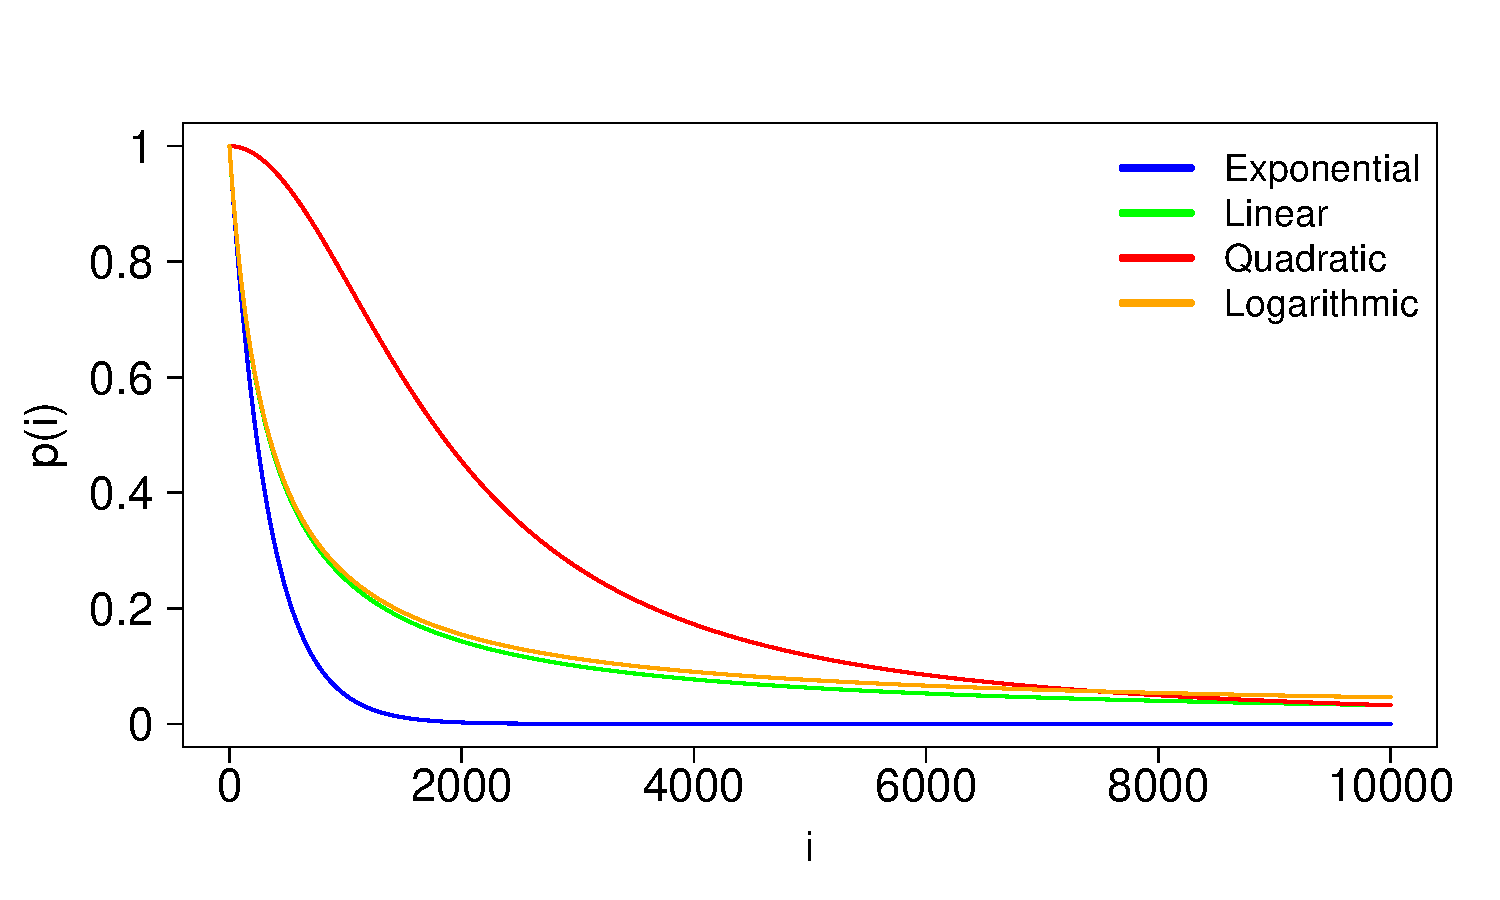
\includegraphics[width=2.3in]{cooling_schedules.pdf}
\caption{
Visualization of four cooling schedule types of Table \ref{tab:cooling_schedules} for probability $p(i)$ of making a 
geometric proposal as a function of the $i$-th MCMC iteration. The displayed schedules have been generated using $a=30$ and 
$b=0$.
}
\label{fig:cooling_schedules}
\end{figure}

\subsection{Expected Complexity}
\label{Expected Complexity}

The concept of complexity carries three distinct meanings in the context of MCMC. Firstly, MCMC methods need to be tuned so
as to achieve a balance between proposing large enough jumps and ensuring that a reasonable proportion of jumps are accepted.
By way of illustration, MALA attains its optimal acceptance rate of $0.574$ as $n_{\theta}\rightarrow\infty$ by setting its
drift step $\epsilon$ to be in the vicinity of $n_{\theta}^{-1/3}$. Because of this, it is said that the algorithmic
efficiency of MALA scales $\mathcal{O}(n_{\theta}^{-1/3})$ as the number $n_{\theta}$ of parameters increases.

Secondly, the quality of MCMC algorithms is assessed by estimating the effective sample size (ESS) of their simulated chains.
The ESS of a chain is interpreted as the number of samples in the chain bearing the same amount of variance as the one found 
in $n_m$ independent samples.

A third criterion for assessing MCMC methods is their computational time.
This criterion corresponds to the ordinary concept of algorithmic complexity as it entails a count of numerical operations
performed by an MCMC algorithm. To give an example, the computational complexity of MALA is of order
$\mathcal{O}(n_{\theta}^2)$ or $\mathcal{O}(n_{\theta})$ depending on the choice of preconditioning matrix, as explained in 
Section \ref{Motivation}.

Of these three indicators of algorithmic complexity, ESS and computational runtime are the ones typically used for
understanding the range of applicability of MCMC methods. To get a single-number summary, the ratio of ESS over runtime is
usually employed. In the present paper, the computational time of ALSMMALA and AMSMMALA are derived theoretically, while both
samplers are empirically assessed in Section \ref{Examples} via their ESS and CPU runtime.

\begin{proposition}
Let $A_1$ and $A_2$ be two MCMC algorithms whose proposal mechanisms have computational complexities $c_1$ and $c_2$, 
respectively. A composite MCMC algorithm $A$ conducts a Bernoulli trial
$B(i)\sim\mbox{Bernoulli}(p(i))~,i\in\left\{1,2,\dots,n_m\right\}$, to take its $i$-th step using the proposal kernel of 
algorithm $A_1$ with probability $p(i)$, or using the proposal mechanism of $A_2$ with probability $1-p(i)$. The mean 
complexity of $A$ is given by
\begin{equation}
\label{eq:c}
\mathcal{O}\left(
\dfrac{\sum_{i=1}^{n_m}p(i)}{n_m}c_1+\dfrac{n_m-\sum_{i=1}^{n_m}p(i)}{n_m}c_2
\right).
\end{equation}
\end{proposition}

\begin{proof}
The expected number of invocations of the proposal kernel associated with algorithm $A_1$ equals 
\begin{equation*}
E\left(\sum_{i=1}^{n_m}B(i)\right)=\sum_{i=1}^{n_m}E(B(i))=\sum_{i=1}^{n_m}p(i),
\end{equation*}
whence the conclusion follows directly.
\end{proof}

\begin{proposition}
If an exponentially decaying schedule $p(i)$, as described by \eqref{exp_schedule_a}, is used for regulating the choice of 
proposal kernel at each step of algorithm $A$, then the expected complexity of $A$ becomes
\begin{equation}
\label{eq:c_exp}
\mathcal{O}\left(
\dfrac{1-\exp{(-a)}}{n_m(1-\exp{(-a/n_m)})}c_1+
\left(1-\dfrac{1-\exp{(-a)}}{n_m(1-\exp{(-a/n_m)})}\right)c_2
\right).
\end{equation}
\end{proposition}

\begin{proof}
Schedule \eqref{exp_schedule_a} yields the geometric series sum
\begin{equation}
\label{eq:c_exp_geom}
\sum_{i=1}^{n_m}p(i)=
\sum_{i=1}^{n_m}\exp{(-a(i-1)/n_m)}=
\dfrac{1-\exp{(-a)}}{1-\exp{(-a/n_m)}}.
\end{equation}
Plugging \eqref{eq:c_exp_geom} into \eqref{eq:c} gives \eqref{eq:c_exp}.
\end{proof}

\begin{lemma}
For sufficiently large number $n_m$ of MCMC iterations ($n_m\rightarrow\infty$), the mean complexity of an algorithm $A$ 
with exponentially decaying schedule \eqref{exp_schedule_a} is.
\begin{equation}
\label{eq:c_exp_limit}
\mathcal{O}\left(
\dfrac{1-\exp{(-a)}}{a}c_1+
\left(1-\dfrac{1-\exp{(-a)}}{a}\right)c_2
\right).
\end{equation}
\end{lemma}

\begin{proof}
It suffices to notice that
\begin{equation}
\lim_{n_m\to\infty}\dfrac{1-\exp{(-a)}}{n_m(1-\exp{(-a/n_m)})}=\dfrac{1-\exp{(-a)}}{a}.
\end{equation}
\end{proof}

\begin{proposition}
The mean complexity of an algorithm $A$ with a $\mod{(a)}$ schedule $p(i)$ is
\begin{equation}
\label{eq:c_mod}
\mathcal{O}\left(
\dfrac{1}{a}c_1+
\dfrac{a-1}{a} c_2
\right).
\end{equation}
\end{proposition}

\begin{proof}
The proposal mechanism of algorithm $c_1$ is called $n_m/a$ times out of $n_m$ iterations. Hence, the proportion of proposals
made via $c_1$ is $1/a$, which completes the proof.
\end{proof}

\begin{lemma}
For a large number $n_m$ of iterations ($n_m\rightarrow\infty$), the expected complexity of ALSMMALA, as presented in 
Algorithm \ref{alsmmala} and equipped with the exponentially decaying schedule defined by \eqref{exp_schedule_a}, is given by
\begin{equation}
\label{eq:c_alsmmala_exp}
\mathcal{O}\left(
\dfrac{1-\exp{(-a)}}{a}n_{\theta}^3+
\left(1-\dfrac{1-\exp{(-a)}}{a}\right)n_{\theta}^2
\right).
\end{equation}
\end{lemma}

\begin{proof}
\eqref{eq:c_alsmmala_exp} follows from \eqref{eq:c_exp_limit} by recalling that the respective complexities of SMMALA and 
MALA are $\mathcal{O}(n_{\theta}^3)$ and $\mathcal{O}(n_{\theta}^2)$.
\end{proof}

\begin{lemma}
The expected complexity of AMSMMALA, as defined in Algorithm \ref{amsmmala}, is
\begin{equation}
\label{eq:c_amsmmala_mod}
\mathcal{O}\left(
\dfrac{1}{a}n_{\theta}^3+
\dfrac{a-1}{a}n_{\theta}^2
\right).
\end{equation}
\end{lemma}

\begin{proof}
Setting $c1=n_{\theta}^3$ and $c_2=n_{\theta}^2$ in \eqref{eq:c_mod}, which correspond to the complexity orders of SMMALA 
and AM, gives \eqref{eq:c_amsmmala_mod}.
\end{proof}

The schedule $p(i)$ for choosing between proposal mechanisms plays a decisive role in the complexity of the resulting sampler
as seen from \eqref{eq:c}. Besides, the decaying rate $a$ of an exponentially decaying schedule \eqref{exp_schedule_a} and 
the modulus $a$ of a $\mod{(a)}$ schedule can be used for adjusting the computational cost according to 
\eqref{eq:c_exp_limit} and \eqref{eq:c_mod}.

Figure \ref{fig:alsmmala_amsmmala_schedule} displays the complexity of ALSMMALA with an exponential schedule specified by
\eqref{exp_schedule_a} and AMSMMALA with a $\mod{(a)}$ schedule as a function of the parameter space dimension $n_{\theta}$.
The curves of Figures \ref{fig:alsmmala_exp_schedule} and \ref{fig:amsmmala_mod_schedule} correspond to varying levels of 
decaying rate $a$ for ALSMMALA and of modulus $a$ for AMSMMALA. In both cases, the tuning factor $a$ determines the 
trade-off between runtime and amount of geometric computation. Larger values of $a$ reduce the runtime due to fewer 
geometric updates, whereas smaller values of $a$ increase the complexity as they induce more geometric updates.

\begin{figure}[t]
	\centering
	\subfloat[ALSMMALA]{
		\label{fig:alsmmala_exp_schedule}
		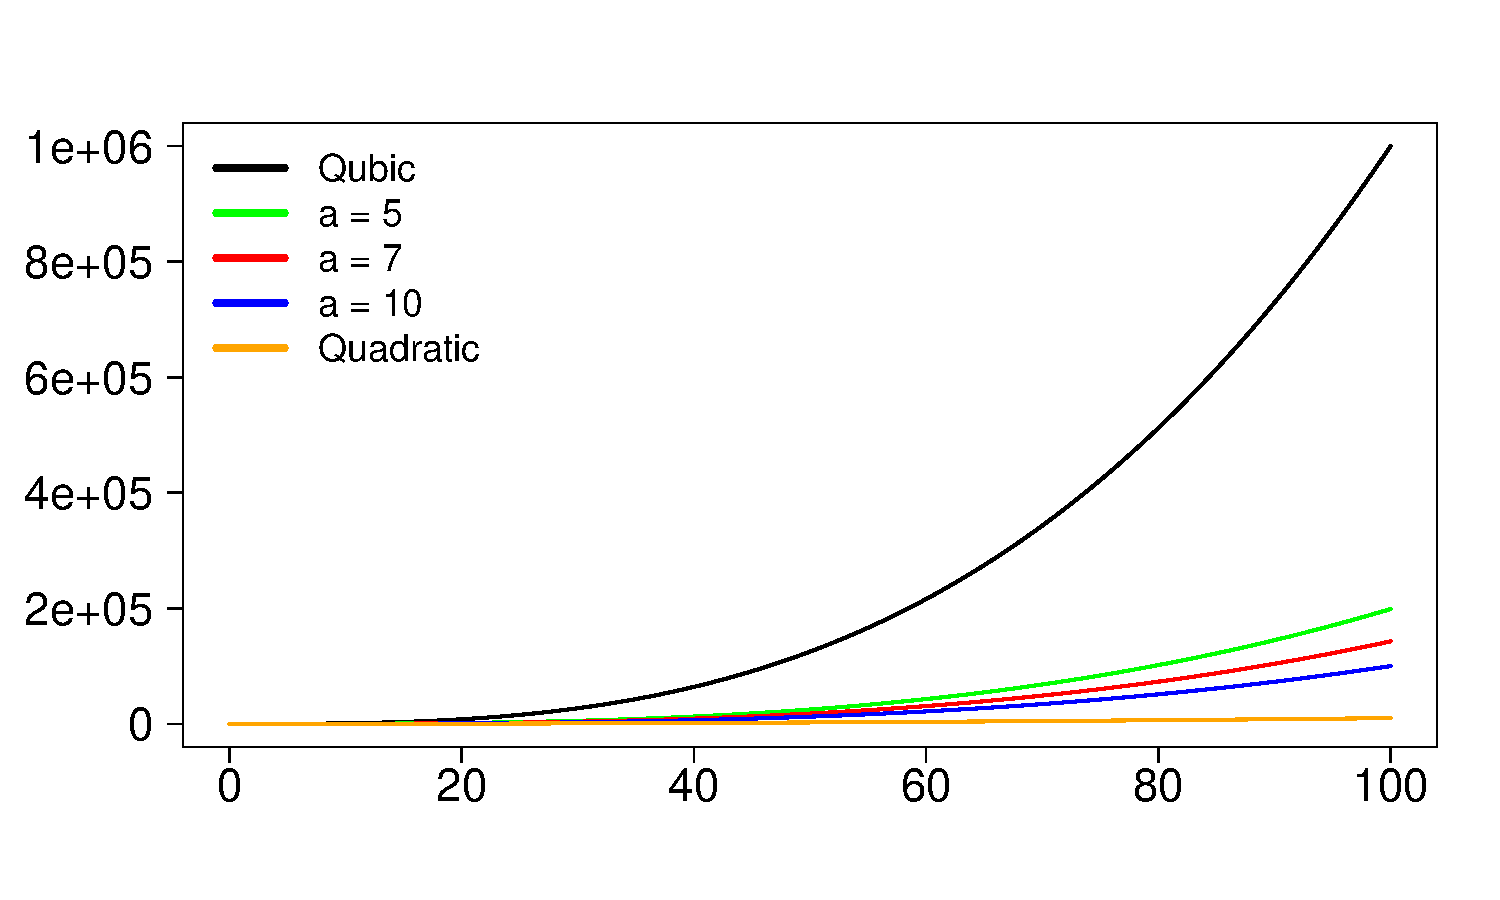
\includegraphics[width=2.3in]{alsmmala_complexity.pdf}
	}
	\subfloat[AMSMMALA]{
		\label{fig:amsmmala_mod_schedule}
		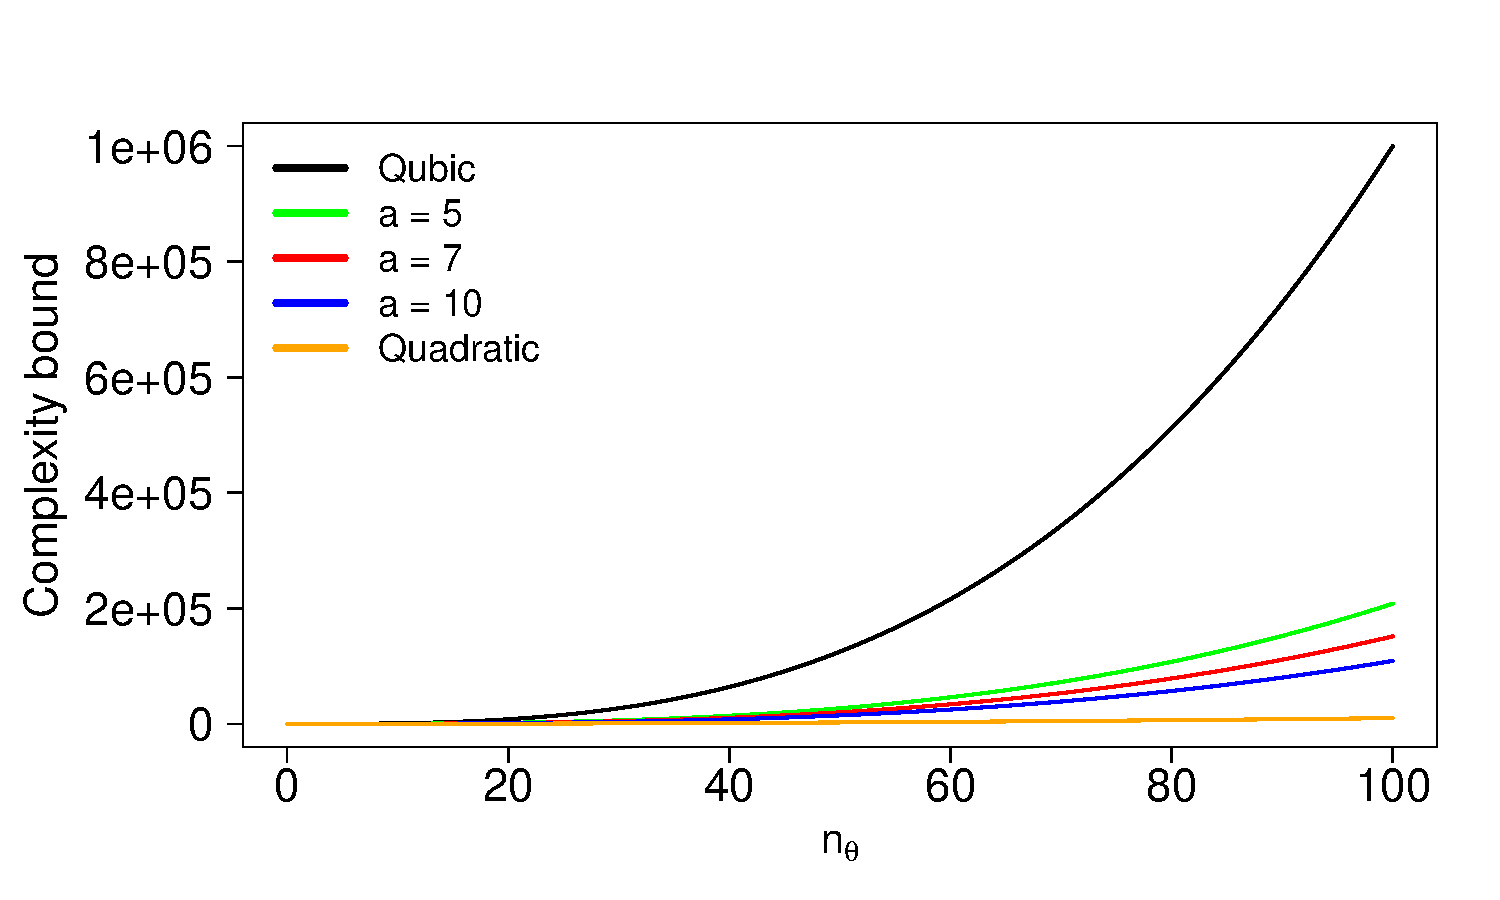
\includegraphics[width=2.3in]{amsmmala_complexity.pdf}
	} \\
	\caption{
		Time complexity of ALSMMALA with an exponential schedule given by \eqref{exp_schedule_a} and AMSMMALA with a $\mod{(a)}$ 
		schedule as a function of the number $n_{\theta}$ of parameters. Different curves correspond to varying levels of 
		decaying rate $a$ for ALSMMALA and of modulus $a$ for AMSMMALA. The qubic complexity of SMMALA and quadratic complexity
		of MALA are displayed as baseline cases.
	}
	\label{fig:alsmmala_amsmmala_schedule}
\end{figure}

\subsection{Analytically Intractable Geometric Updates}

In practice, challenges in the implementation of manifold MCMC algorithms might raise additional computational implications.
In particular, two notoriously incurring issues relate to the Cholesky decomposition of metric $G^{-1}(\boldsymbol{\theta})$ 
and to the calculation of up to third order derivatives of $G(\boldsymbol{\theta})$.

Various contributing factors, including finite-precision floating point arithmetic, can lead to an indefinite proposal
covariance matrix $\epsilon^2 G^{-1}(\boldsymbol{\theta})$. This in turn breaks the Cholesky factorization of 
$\epsilon^2 G^{-1}(\boldsymbol{\theta})$. \cite{bet__age} introduced the so-called SoftAbs metric, which offers a 
positive-definite approximation of the indefinite proposal covariance. The working SoftAbs solution to the Cholesky 
factorization problem involves an eigen-decomposition, so it comes with an $\mathcal{O}(n_{\theta}^3)$ cost.

Non-trivial models can render the analytic derivation of log-target derivatives impossible or impractical. Automatic
differentiation (AD), a computationally driven research activity that has evolved since the mid 1950's, helps compute 
derivatives in a numerically exact way. Indeed, \cite{gri__ona} has shown that AD is backward stable in the sense of 
\cite{wil__mod}. Thus, small perturbations of the original function due to machine precision still yield accurate 
derivatives calculated via AD.

There are different methods of automatic differentiation; reverse mode AD is better suited for functions
$f:\mathbb{R}^n\rightarrow\mathbb{R}$, in contrast to forward mode AD that is more suitable for functions 
$f:\mathbb{R}\rightarrow\mathbb{R}^n$ (\cite{gri_wal__eva}). Consequently, reverse mode AD is utilized for computing 
derivatives of probability distributions, and finds use in statistical inference. The complexity of reverse mode AD is not
worse than that of the respective analytical derivatives of a target density, assuming of course a carefully crafted
implementation.

\section{Examples}
\label{Examples}

ALSMMALA and AMSMMALA are put to test via three examples to empirically validate these two MCMC algorithms and to assess 
their computational efficacy. Ten chains are simulated from each sampler of each example. $110,000$ iterations are run for 
the realization of each chain, of which the first $10,000$ burn-in are discarded, so $n_m=100,000$ MCMC samples are retained.

The effective sample size (ESS) of each dimension $\boldsymbol{\theta}_{(i)},~i\in\left\{1,2,\dots,n_{\theta}\right\}$,
of the parameter vector $\boldsymbol{\theta}$ is computed as
\begin{equation}
\mbox{ESS} =
\dfrac{n_m\hat{\sigma}^2_{IID}}{\hat{\sigma}^2_{MCMC}},
\end{equation}
where $\hat{\sigma}^2_{IID}$ and $\hat{\sigma}^2_{MCMC}$ denote the ordinary and Monte Carlo variance of the associated 
chain. The Monte Carlo variance $\hat{\sigma}^2_{MCMC}$ is calculated by means of the initial monotone sequence estimator of
\cite{gey__pra}. To get more reliable estimates, the ESS of each dimension and the CPU runtime are averaged by taking their
respective means across every set of ten chains simulated from a sampler. The computational efficiency of each sampler is
defined as the ratio $\min\left\{\mbox{ESS}_i:i=1,2,\dots,n_{\theta}\right\}/\mbox{time}$ of the smallest ESS
$\min\left\{\mbox{ESS}_i:i=1,2,\dots,n_{\theta}\right\}$ among all $n_{\theta}$ dimensions over the simulation time. Finally,
the relative speed-up of one MCMC method over another is set to be the ratio of their computational efficiencies.

A package, called PGUManifoldMC, has been developed to implement ALSMMALA and AMSMMALA using the Julia programming language.
PGUManifoldMC is based on Lora, a package for MCMC inference written in Julia by one of the two authors. PGUManifoldMC is
publicly available at \url{https://github.com/scidom/PGUManifoldMC.jl} under an MIT license. The PGUManifoldMC package ships
with the three examples of this paper.

\newpage
\subsection{Bayesian Logistic Regression}

\begin{table}
	\caption{Logistic regression - comparison of Langevin sampling methods}
	\label{tab:logit}
	\begin{tabular}{l|r|rrrr|r|r|r}
		\hline\noalign{\smallskip}
		\multirow{2}{*}{Method} &
		\multirow{2}{*}{AR} &
		\multicolumn{4}{c|}{ESS} &
		\multirow{2}{*}{Time} &
		\multirow{2}{*}{Efficiency} &
		\multirow{2}{*}{Speedup} \\
		& & $\theta_1$ & $\theta_2$ & $\theta_3$ & $\theta_4$ & & & \\
		\noalign{\smallskip}\hline\noalign{\smallskip}
		MALA & .60 & 23077 & 8039 & 8892 & 8562 & 3.05 & 2637.47 & 1.00 \\
		SMMALA & .69 & 15138 & 15246 & 15098 & 12989 & 6.78 & 1916.05 & 0.73 \\
		AMSMMALA & .25 & 9401 & 9208 & 9366 & 8803 & 3.84 & 2291.60 & 0.87 \\
	  ALSMMALA & .63 & 31562 & 31046 & 30656 & 26535 & 4.82 & 5503.74 & 2.09 \\
		\noalign{\smallskip}\hline
	\end{tabular}
\end{table}

\begin{figure}
	\centering
	\subfloat[Running mean]{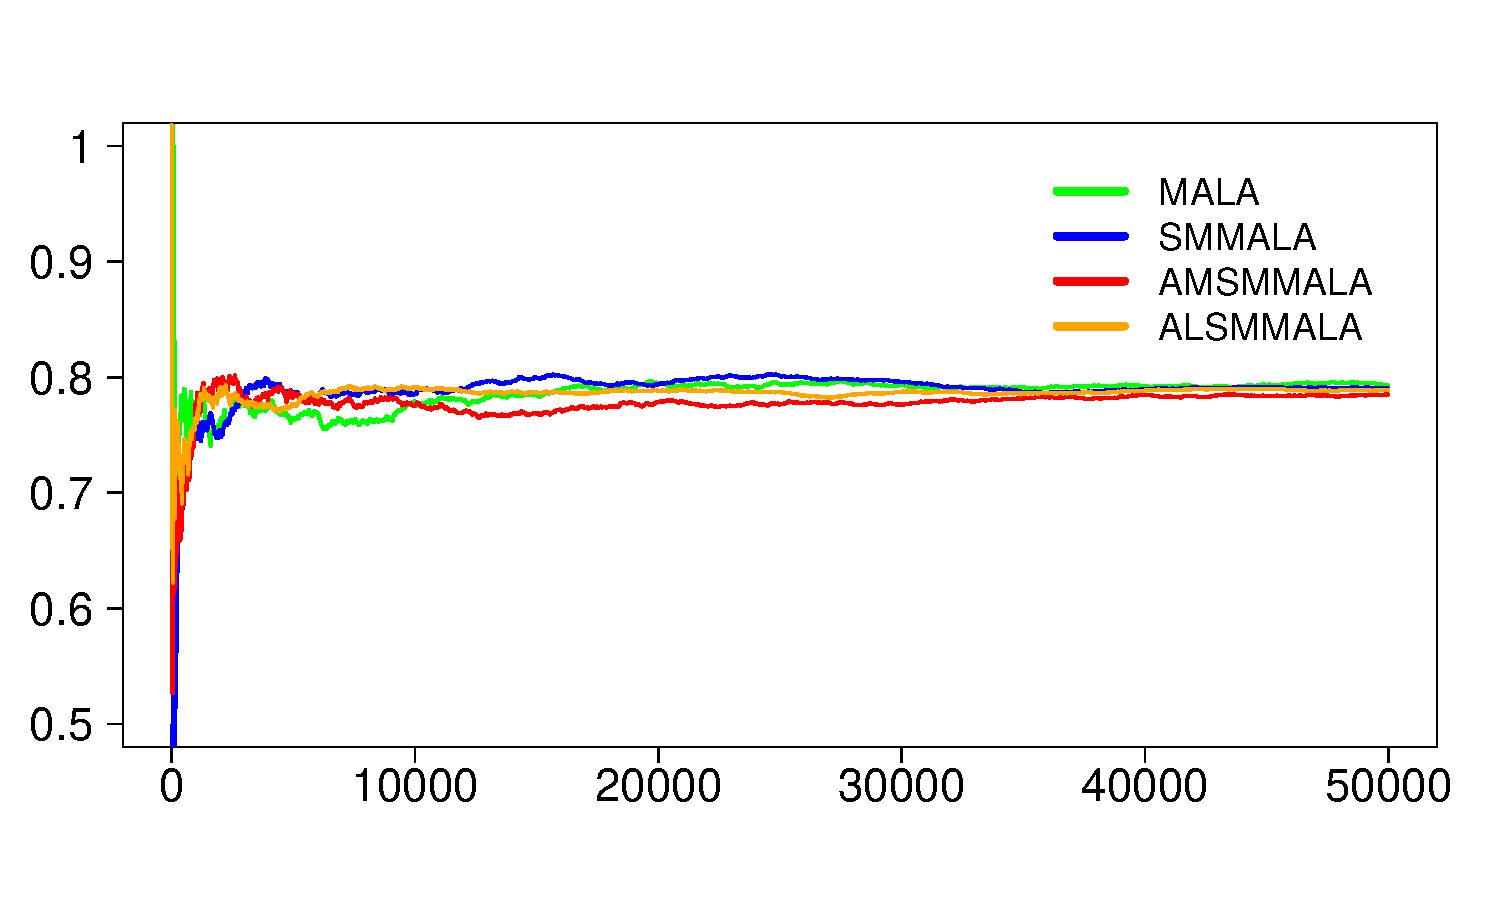
\includegraphics[width=2.3in]{logit_meanplot.pdf}} 
	\subfloat[Linear ACF]{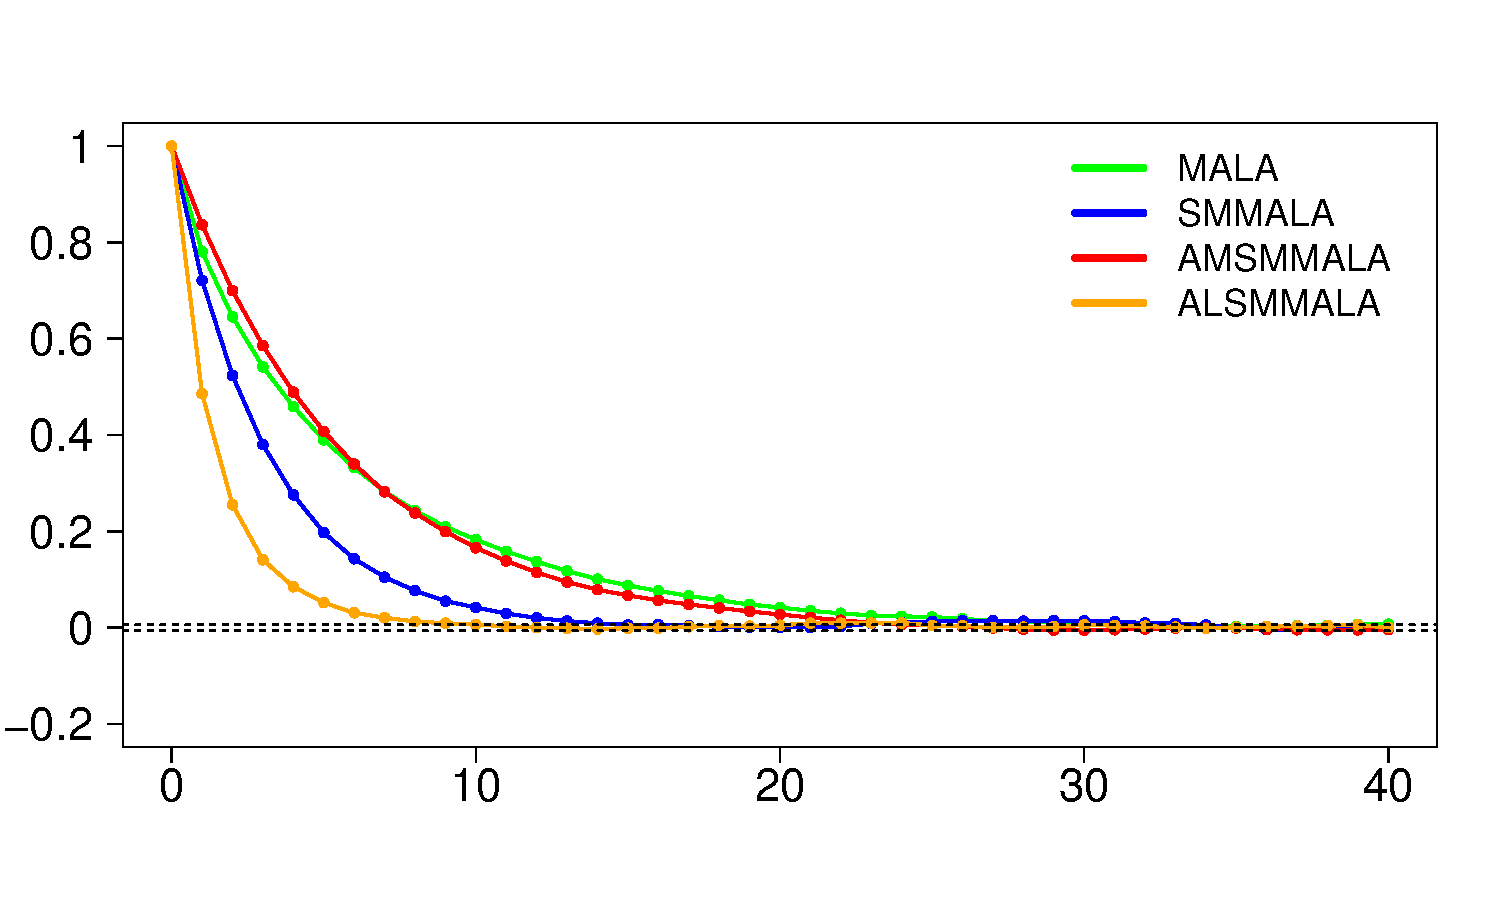
\includegraphics[width=2.3in]{logit_acfplot.pdf}} \\
	\subfloat[MALA traceplot]{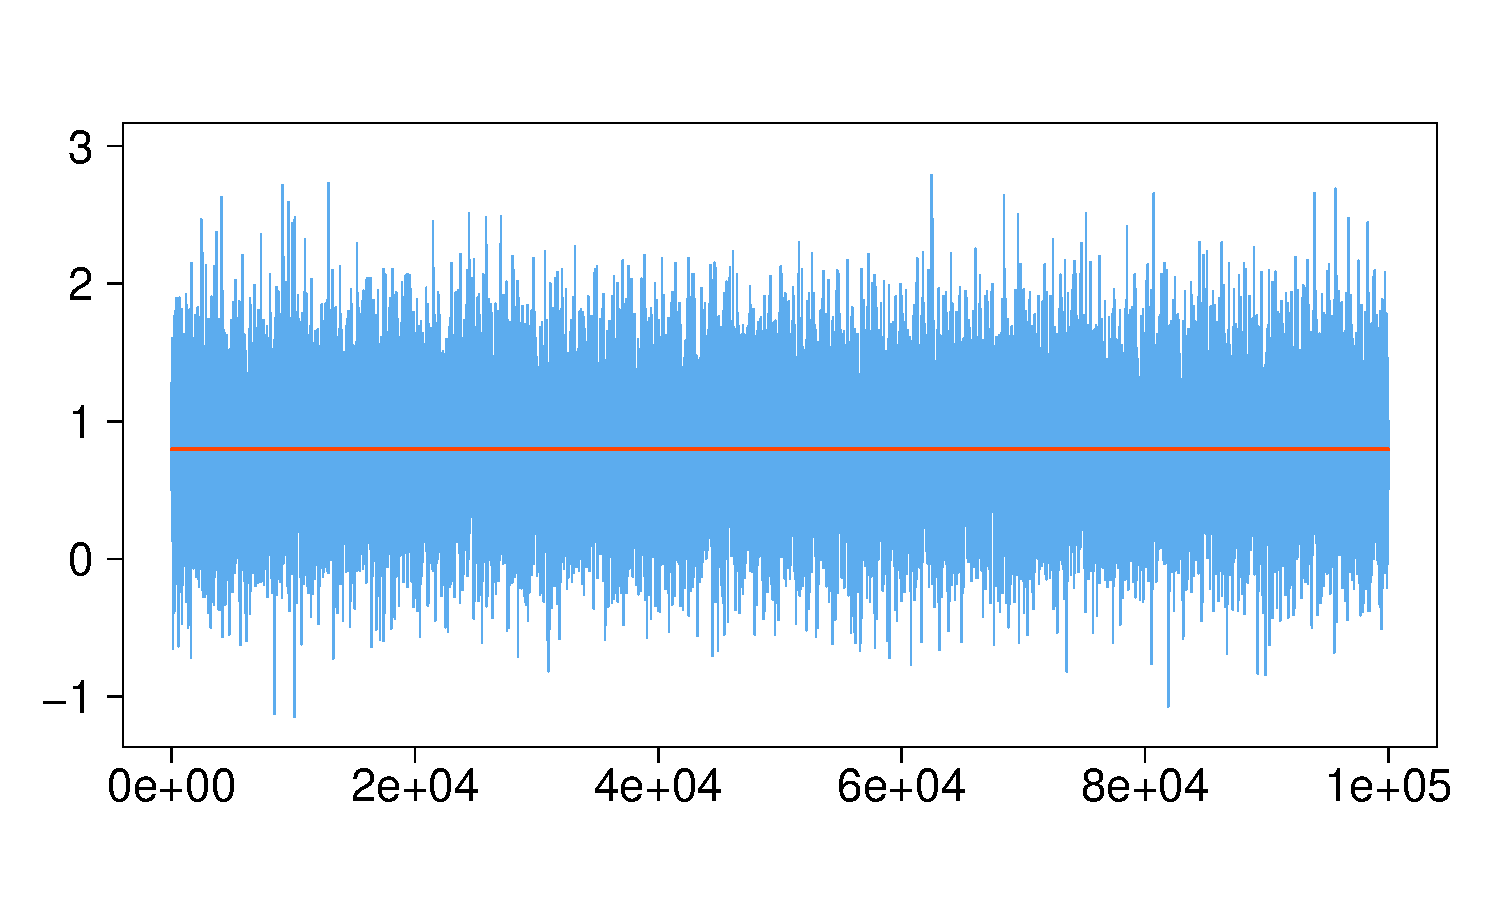
\includegraphics[width=2.3in]{logit_mala_traceplot.pdf}} 
	\subfloat[SMMALA traceplot]{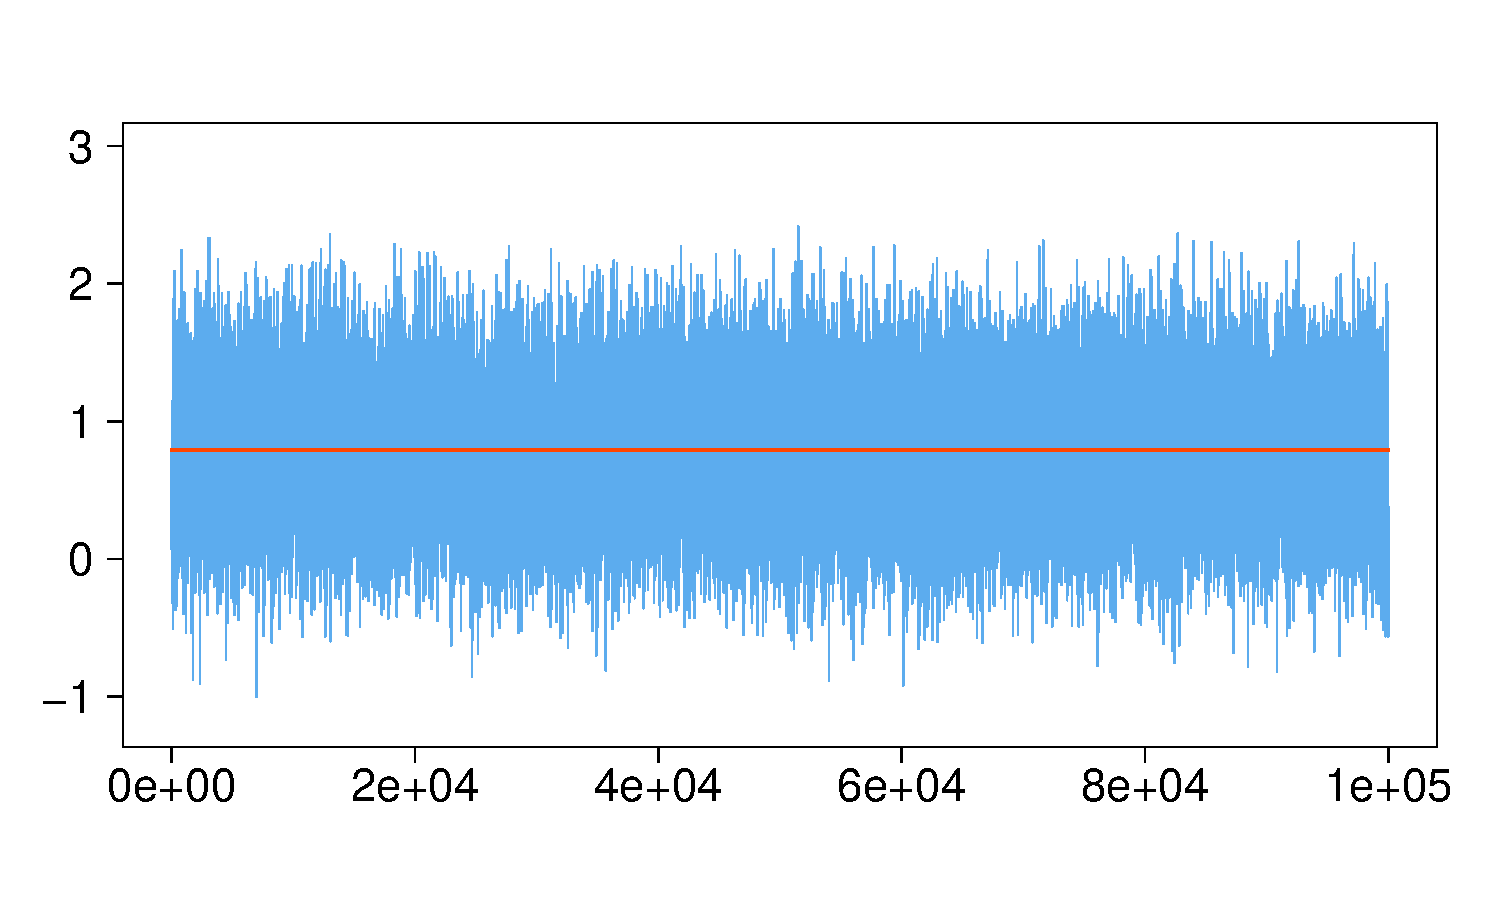
\includegraphics[width=2.3in]{logit_smmala_traceplot.pdf}} \\
	\subfloat[AMSMMALA traceplot]{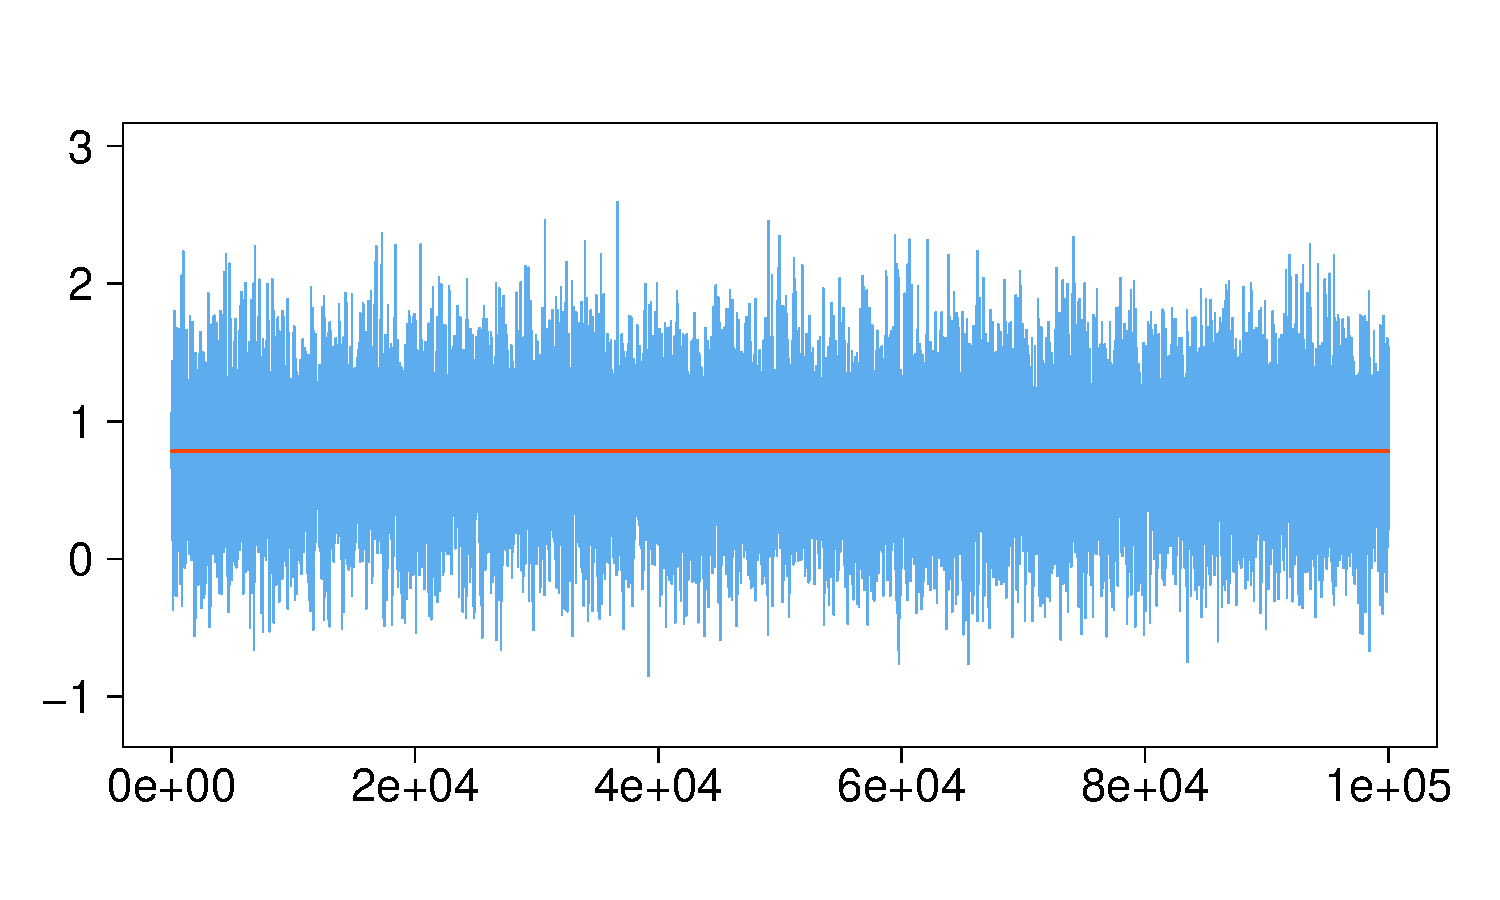
\includegraphics[width=2.3in]{logit_amsmmala_traceplot.pdf}}
	\subfloat[ALSMMALA traceplot]{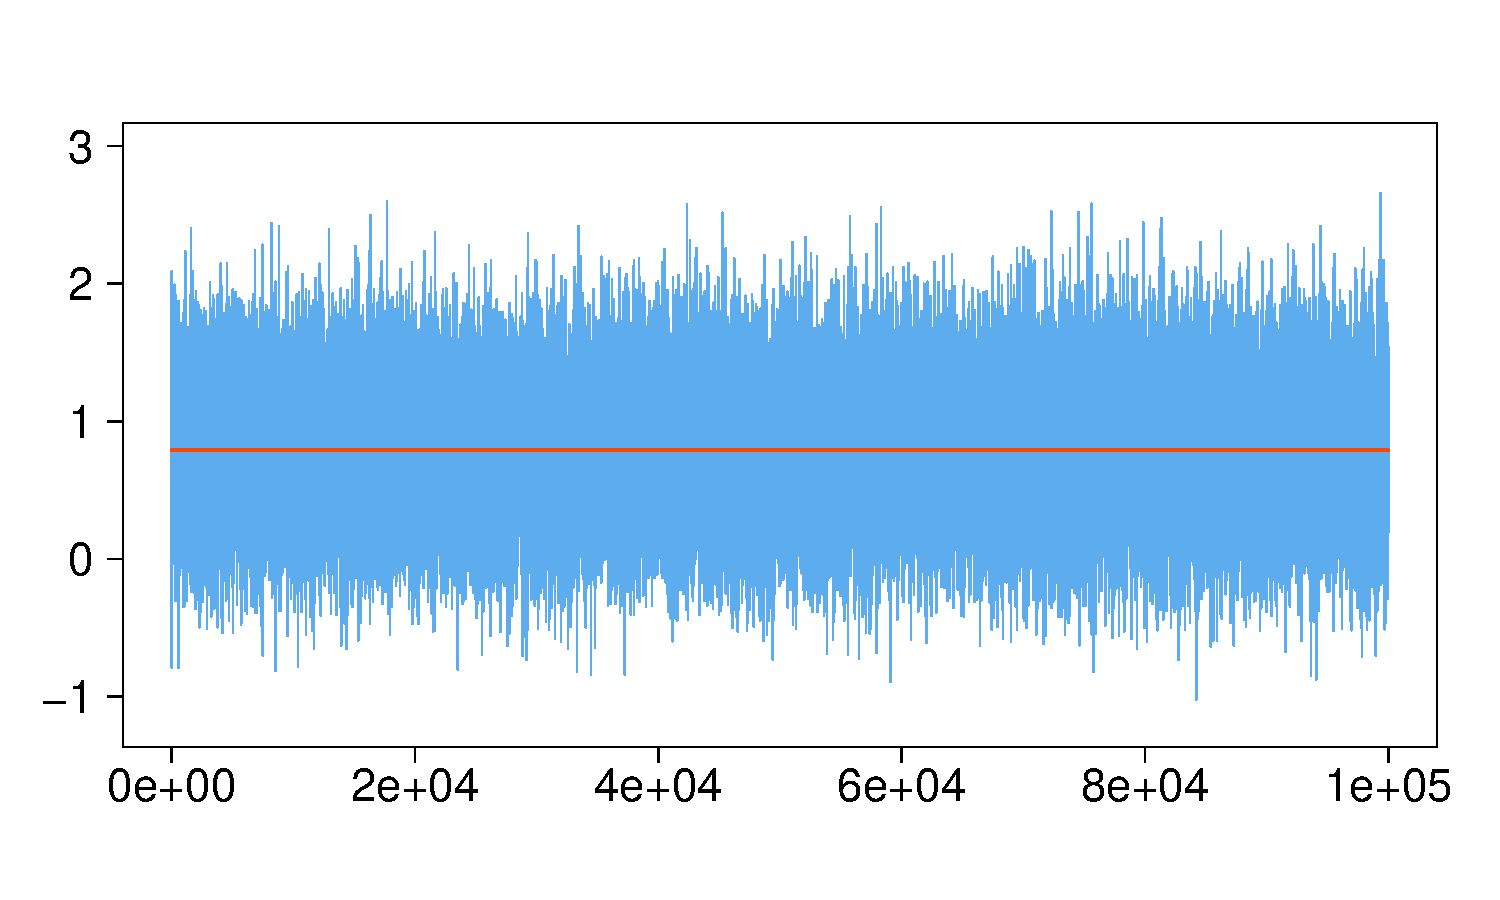
\includegraphics[width=2.3in]{logit_alsmmala_traceplot.pdf}} \\
	\caption{Logistic regression - plots}
	\label{fig:logit}
\end{figure}

\newpage
\subsection{Bayesian Poisson Regression}

\begin{table}
	\caption{Poisson regression - comparison of Langevin sampling methods}
	\label{tab:poisson}
	\begin{tabular}{l|r|rrrr|r|r|r}
		\hline\noalign{\smallskip}
		\multirow{2}{*}{Method} &
		\multirow{2}{*}{AR} &
		\multicolumn{4}{c|}{ESS} &
		\multirow{2}{*}{Time} &
		\multirow{2}{*}{Efficiency} &
		\multirow{2}{*}{Speedup} \\
		& & $\theta_1$ & $\theta_2$ & $\theta_3$ & $\theta_4$ & & & \\
		\noalign{\smallskip}\hline\noalign{\smallskip}
		MALA & .60 & 12649 & 14519 & 12942 & 32161 & 2.36 & 5354.88 & 1.00 \\
		SMMALA & .71 & 40132 & 39657 & 39522 & 39552 & 5.48 & 7212.76 & 1.35 \\
		AMSMMALA & .26 & 11825 & 11667 & 11530 & 11820 & 3.12 & 3692.49 & 0.69 \\
		ALSMMALA & .60 & 43157 & 43089 & 42892 & 43249 & 3.83 & 11194.52 & 2.09 \\
		\noalign{\smallskip}\hline
	\end{tabular}
\end{table}

\begin{figure}
	\centering
	\subfloat[Running mean]{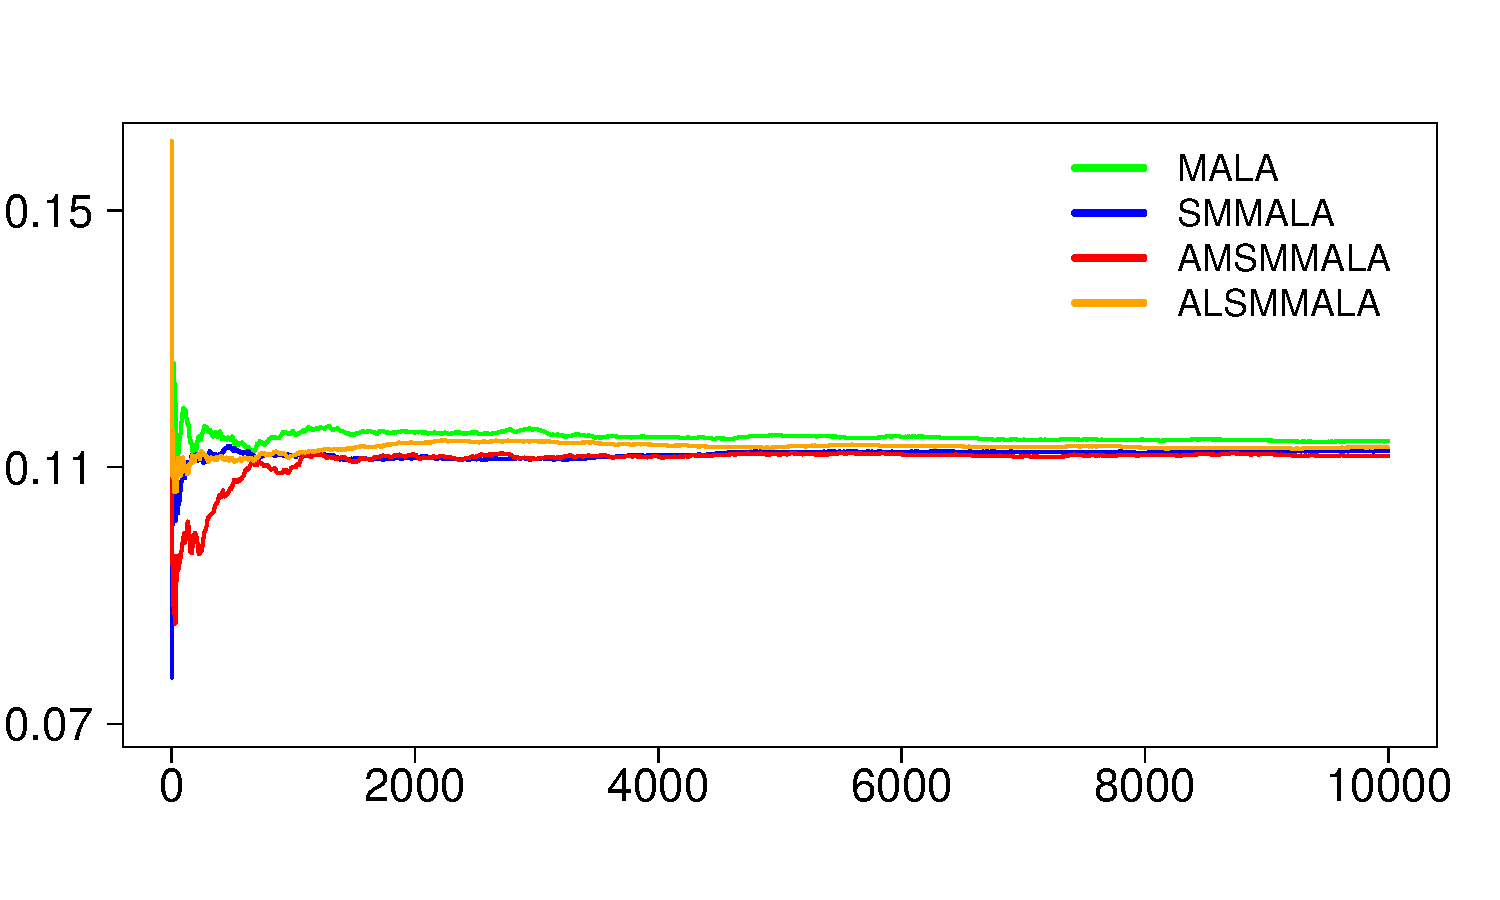
\includegraphics[width=2.3in]{poisson_meanplot.pdf}} 
	\subfloat[Linear ACF]{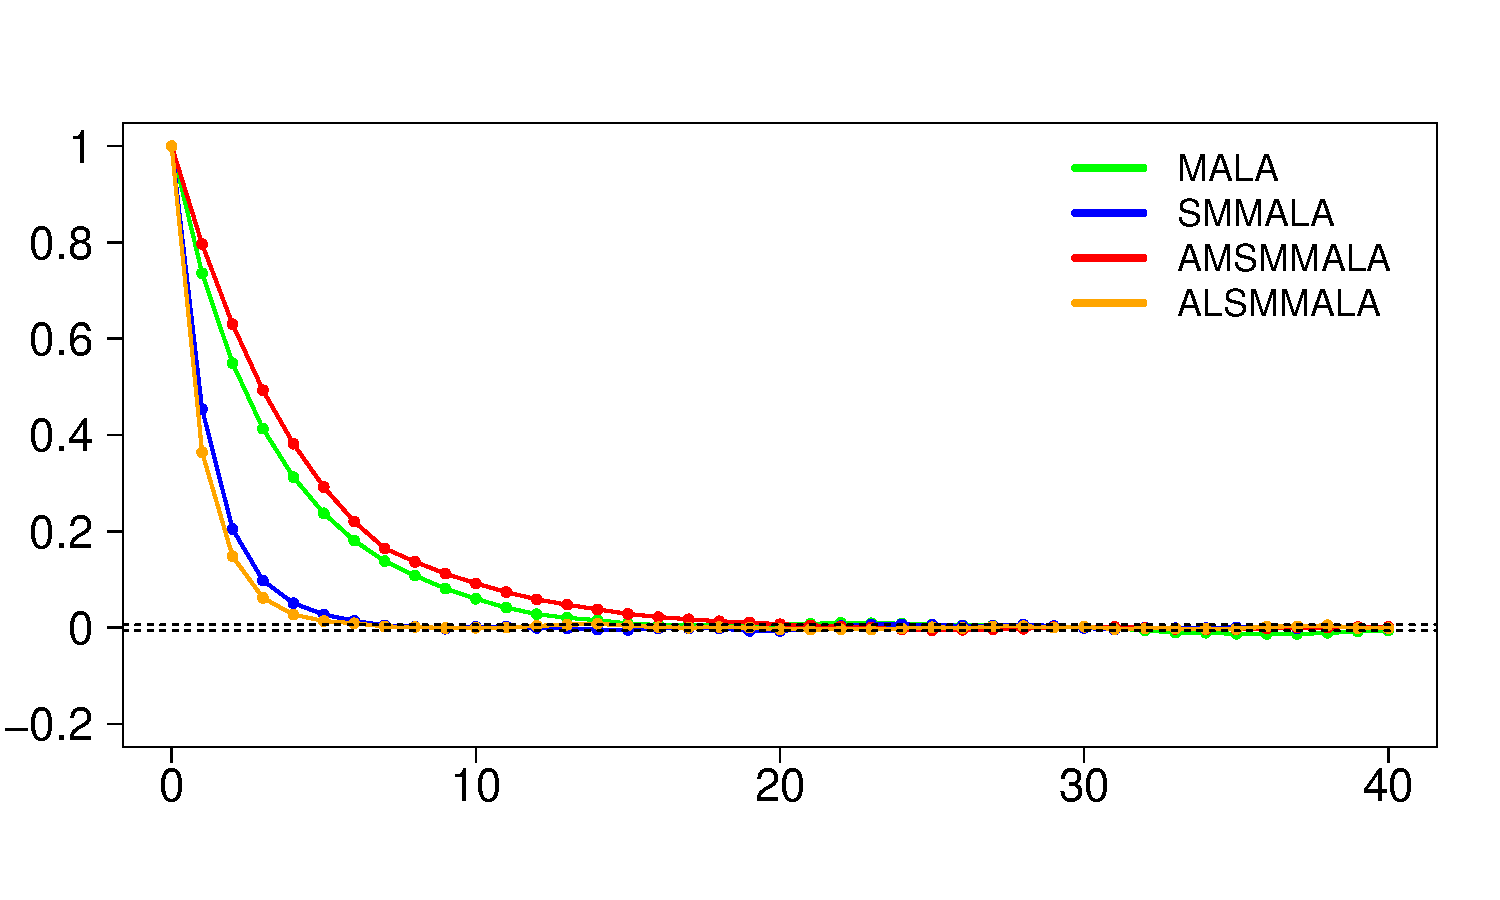
\includegraphics[width=2.3in]{poisson_acfplot.pdf}} \\
	\subfloat[MALA traceplot]{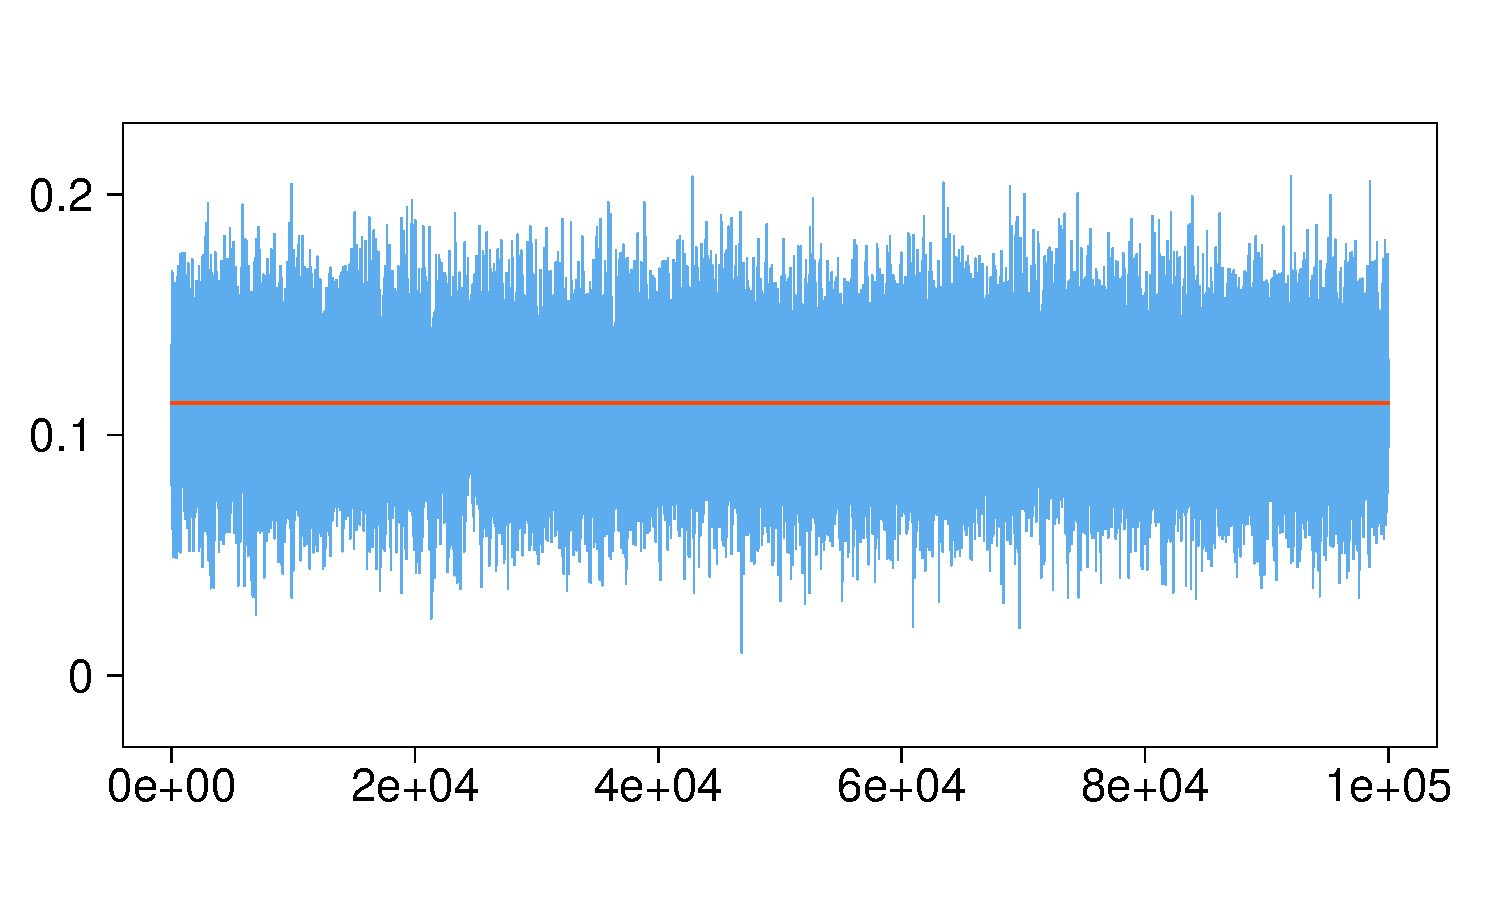
\includegraphics[width=2.3in]{poisson_mala_traceplot.pdf}} 
	\subfloat[SMMALA traceplot]{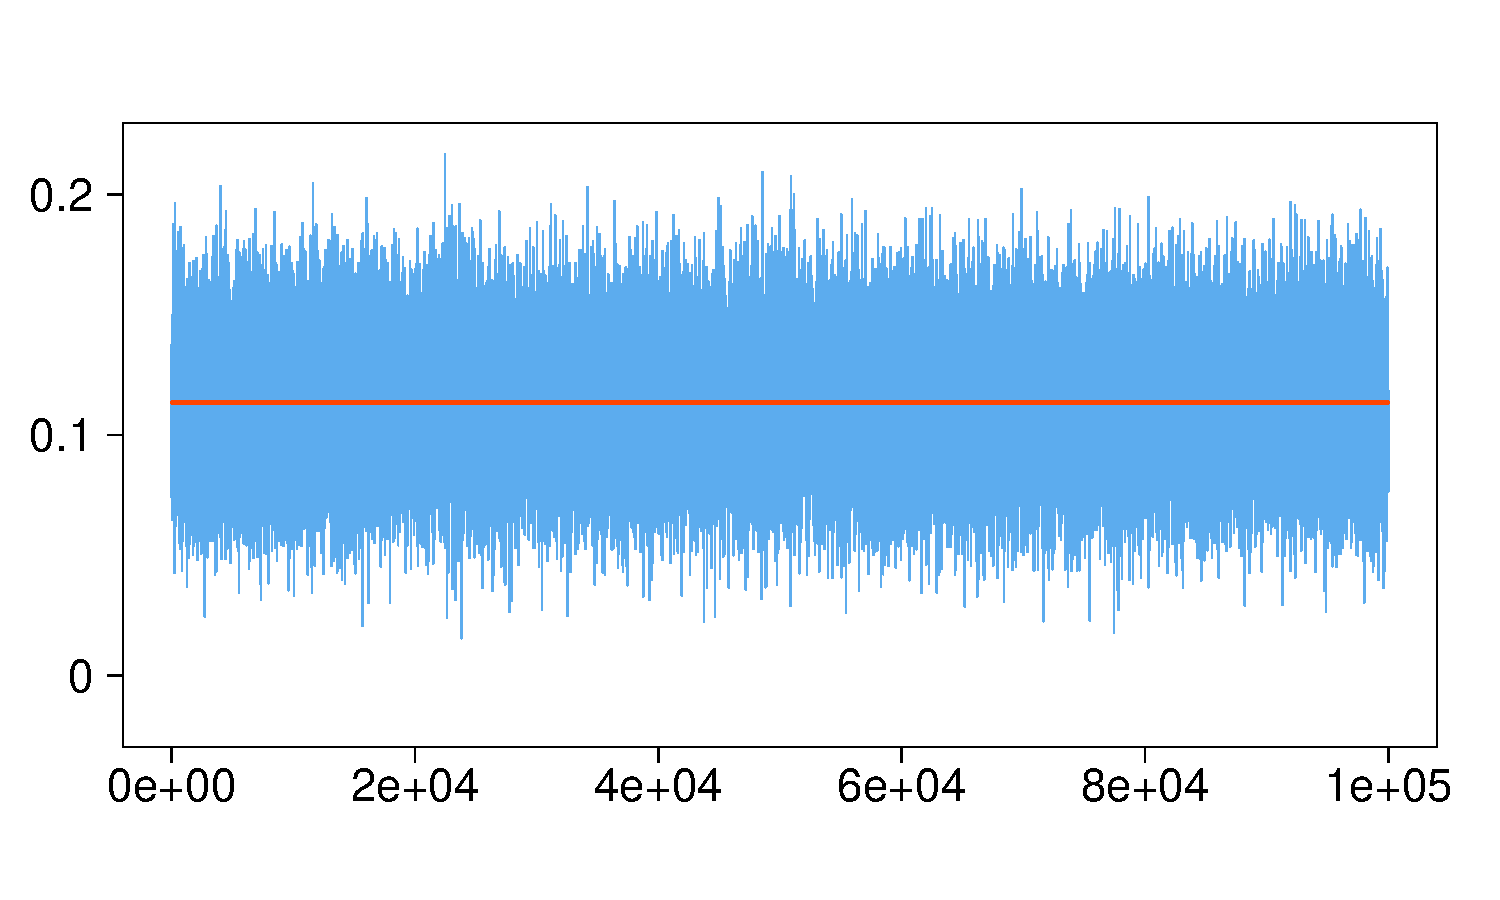
\includegraphics[width=2.3in]{poisson_smmala_traceplot.pdf}} \\
	\subfloat[AMSMMALA traceplot]{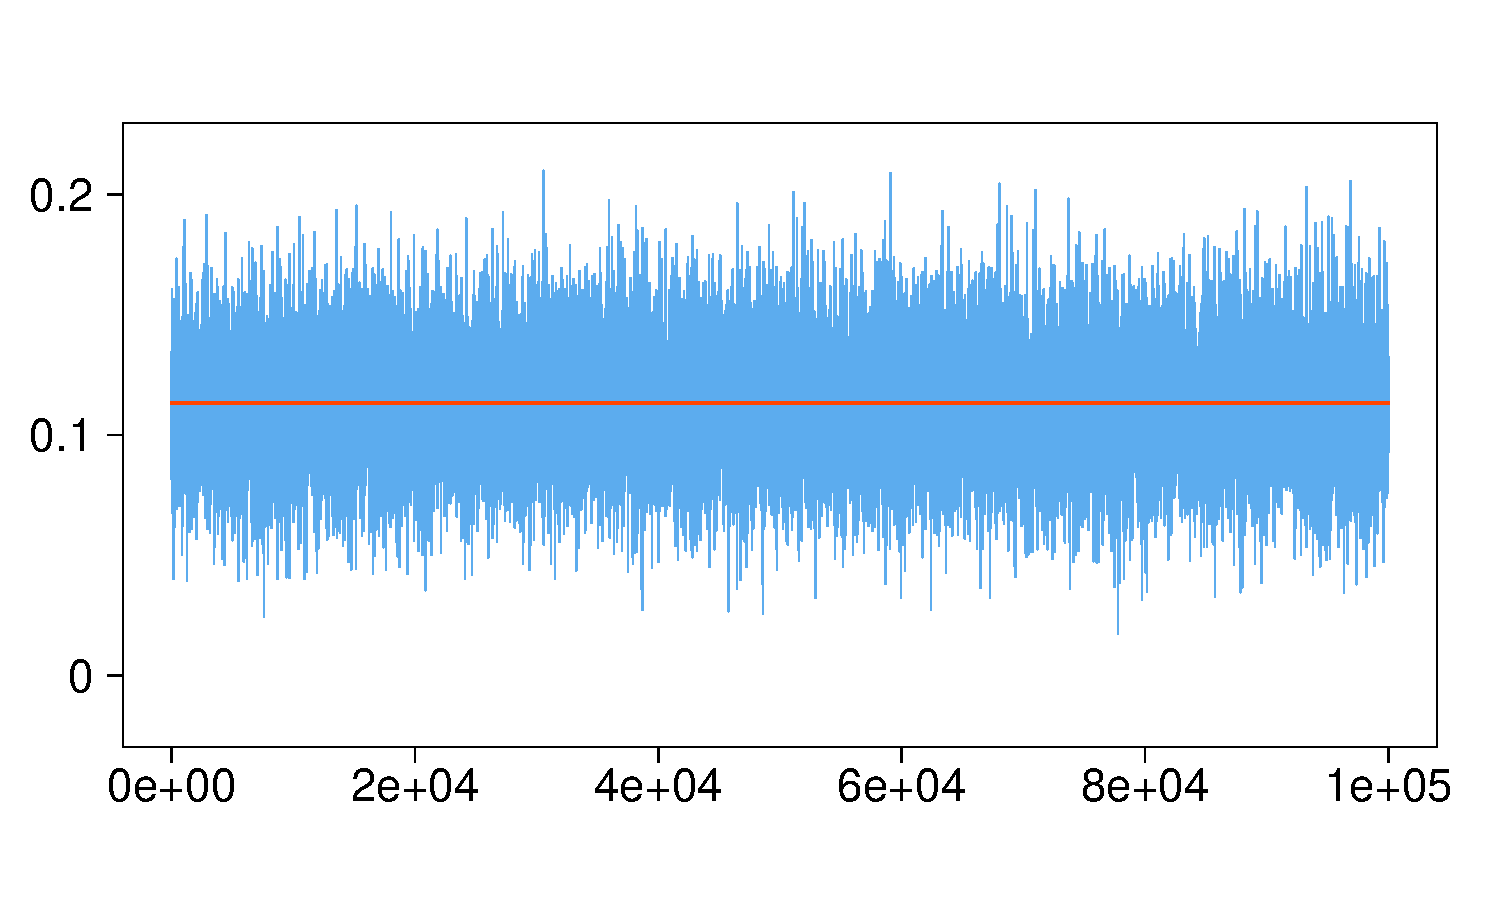
\includegraphics[width=2.3in]{poisson_amsmmala_traceplot.pdf}}
	\subfloat[ALSMMALA traceplot]{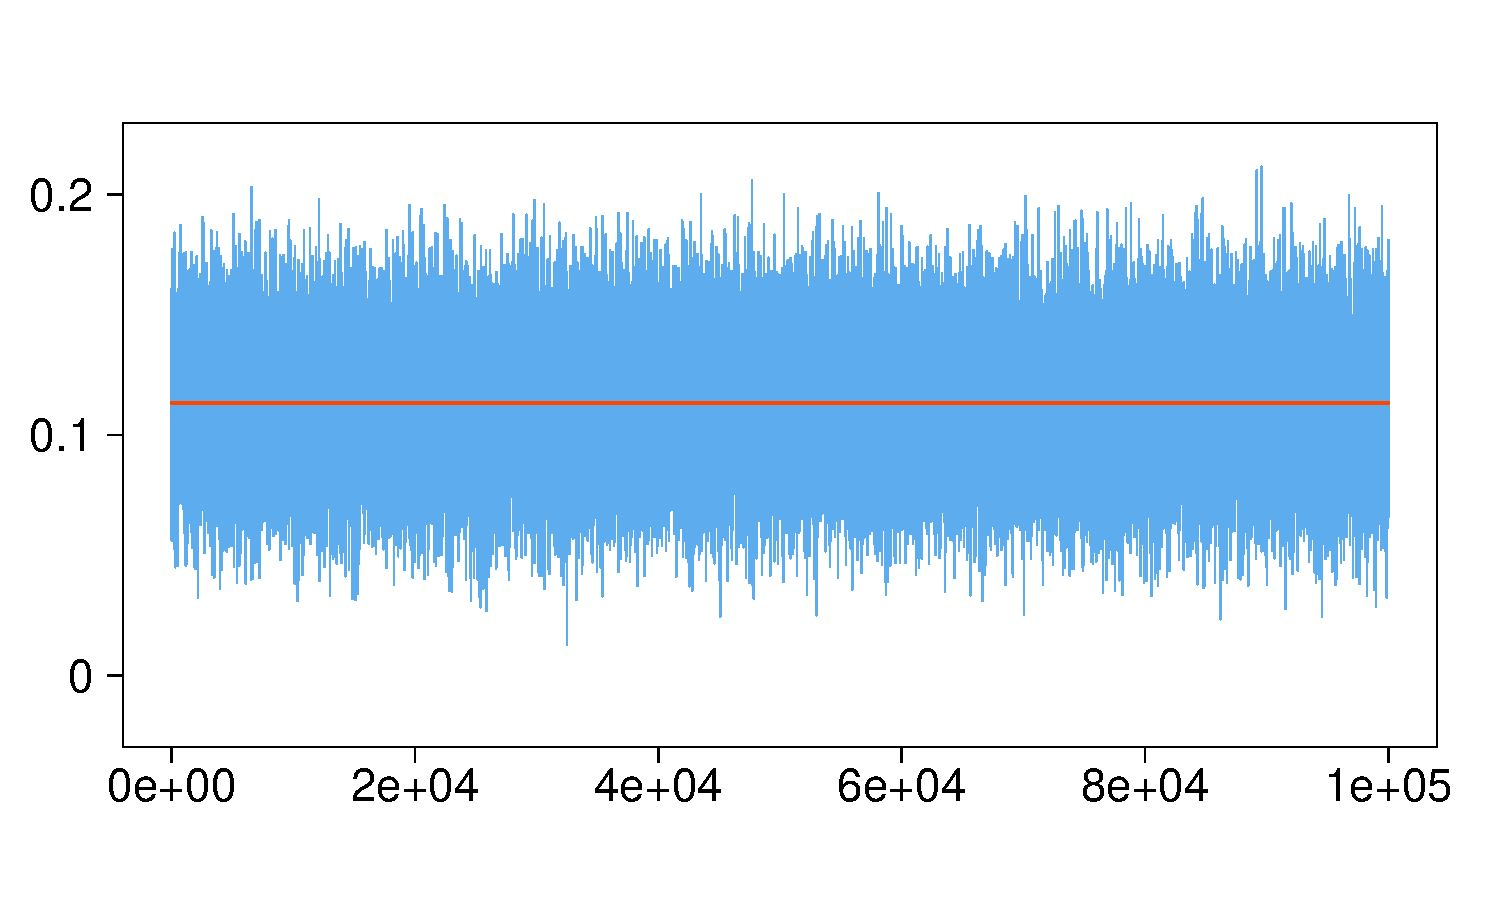
\includegraphics[width=2.3in]{poisson_alsmmala_traceplot.pdf}} \\ 
	\caption{Poisson regression - plots}
	\label{fig:poisson}
\end{figure}

\newpage
\subsection{Multivariate t-Distribution}

Mention that the base algorithm drives the simulation and sets the properties of the sampler. For this reason AMSMMALA works
better than ALSMMALA for the t-dist example. Reference ForwardDiff conference paper, \cite{rev_lub_pap__for}.

\begin{table}
	\caption{t-density target - comparison of Langevin sampling methods. SMMALA (r) is SMMALA with reverse mode AD, and 
	SMMALA (f) is SMMALA with forward mode AD}
	\label{tab:t}
	\begin{tabular}{l|r|rrr|r|r|r}
		\hline\noalign{\smallskip}
		\multirow{2}{*}{Method} &
		\multirow{2}{*}{AR} &
		\multicolumn{3}{c|}{ESS} &
		\multirow{2}{*}{Time} &
		\multirow{2}{*}{Efficiency} &
		\multirow{2}{*}{Speedup} \\
		& & mean & median & max & & & \\
		\noalign{\smallskip}\hline\noalign{\smallskip}
		MALA & .60 & 127 & 145 & 239 & 1.95 & 65.09 & 1.00 \\
		SMMALA (r) & .67 & 103 & 114 & 123 & 41.39 & 2.48 & 0.04 \\
		SMMALA (f) & .68 & 97 & 104 & 121 & 575.29 & 0.17 & 0.00 \\
		AMSMMALA & .16 & 7753 & 7866 & 7960 & 15.27 & 507.74 & 7.80 \\
		ALSMMALA & .96 & 2465 & 2538 & 2574 & 16.16 & 152.51 & 2.34 \\	
		\noalign{\smallskip}\hline
	\end{tabular}
\end{table}

\begin{figure}
	\centering
	\subfloat[Running mean]{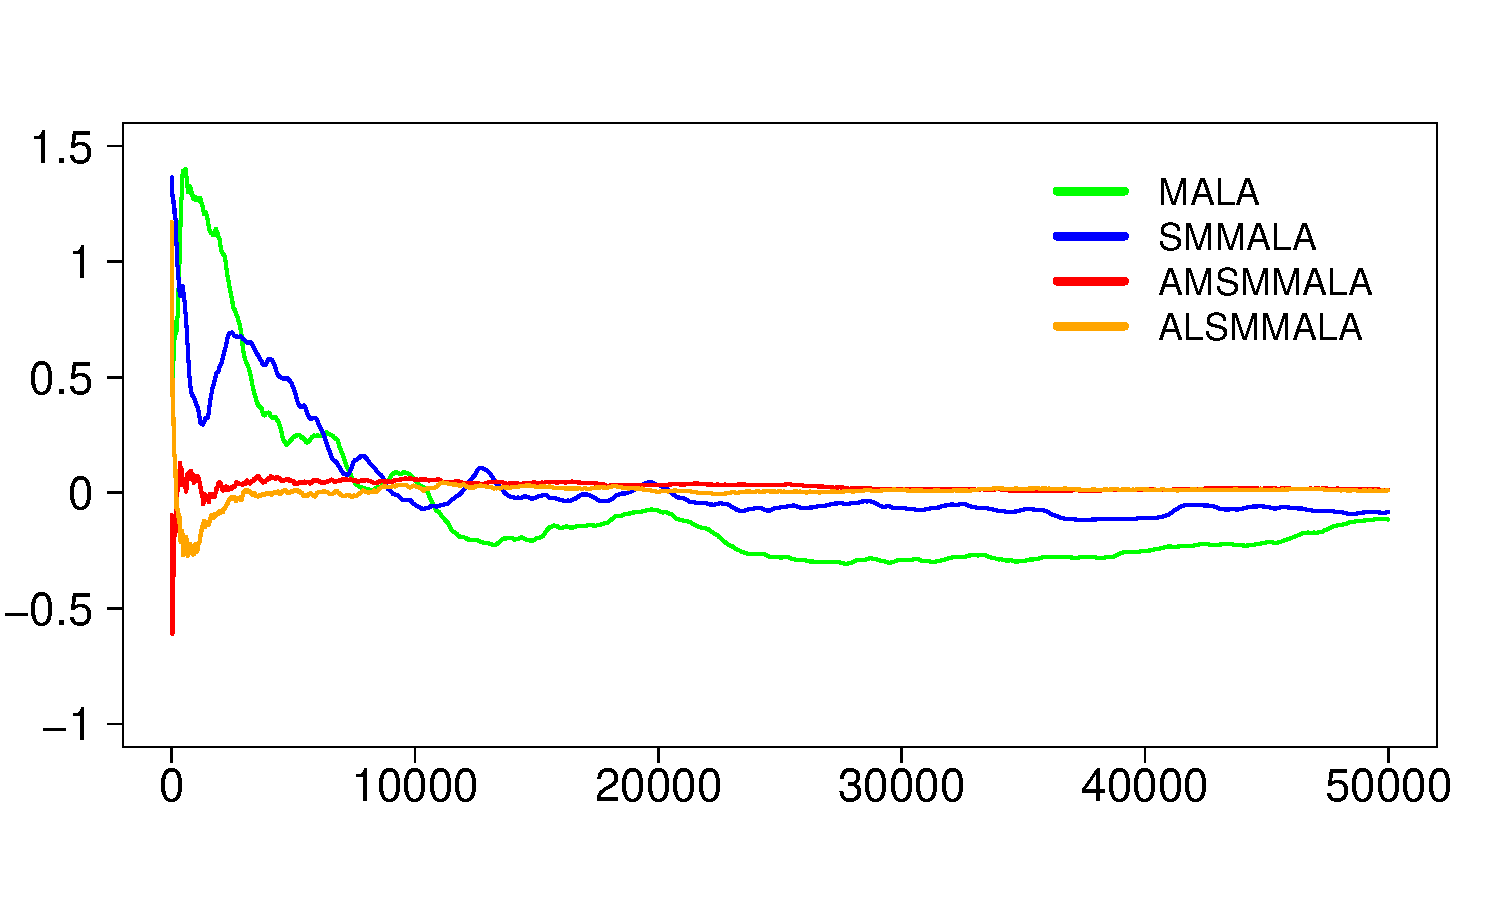
\includegraphics[width=2.3in]{tdist_meanplot.pdf}} 
	\subfloat[Linear ACF]{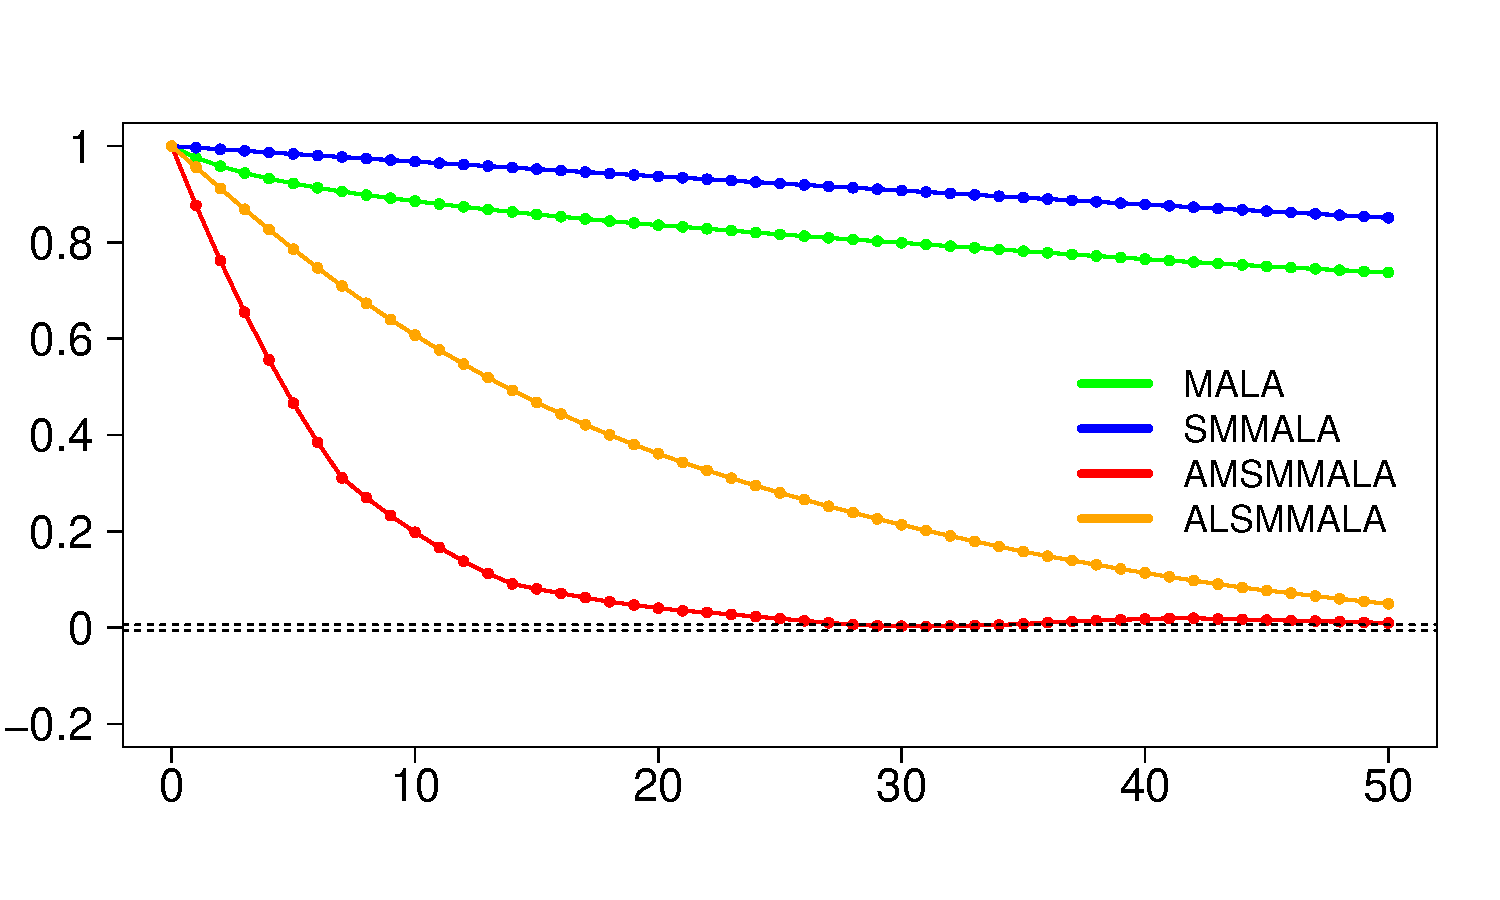
\includegraphics[width=2.3in]{tdist_acfplot.pdf}} \\
	\subfloat[MALA traceplot]{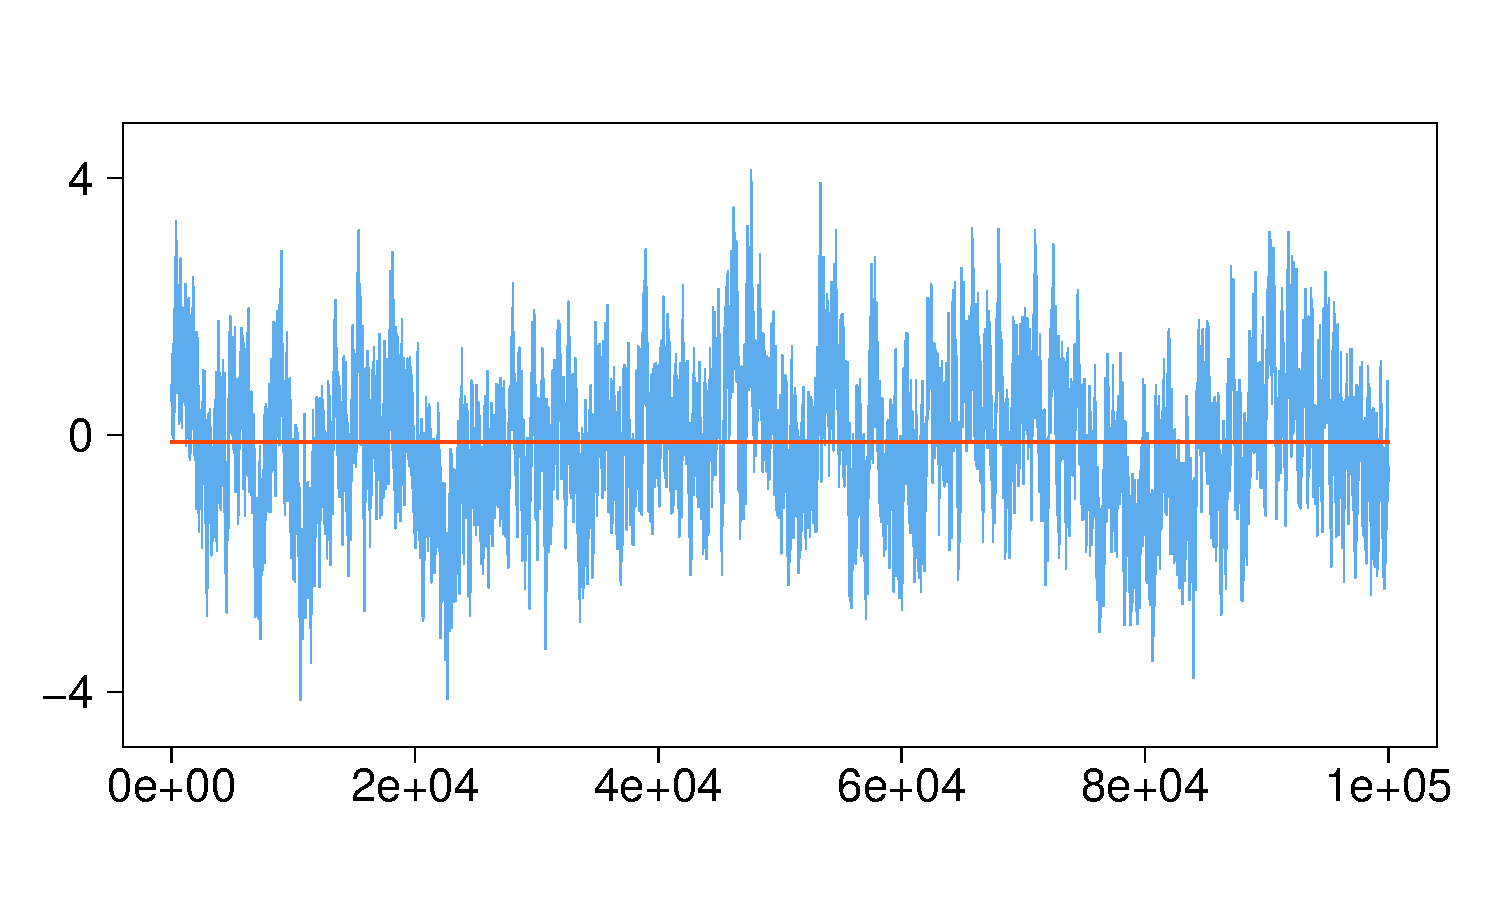
\includegraphics[width=2.3in]{tdist_mala_traceplot.pdf}} 
	\subfloat[SMMALA traceplot]{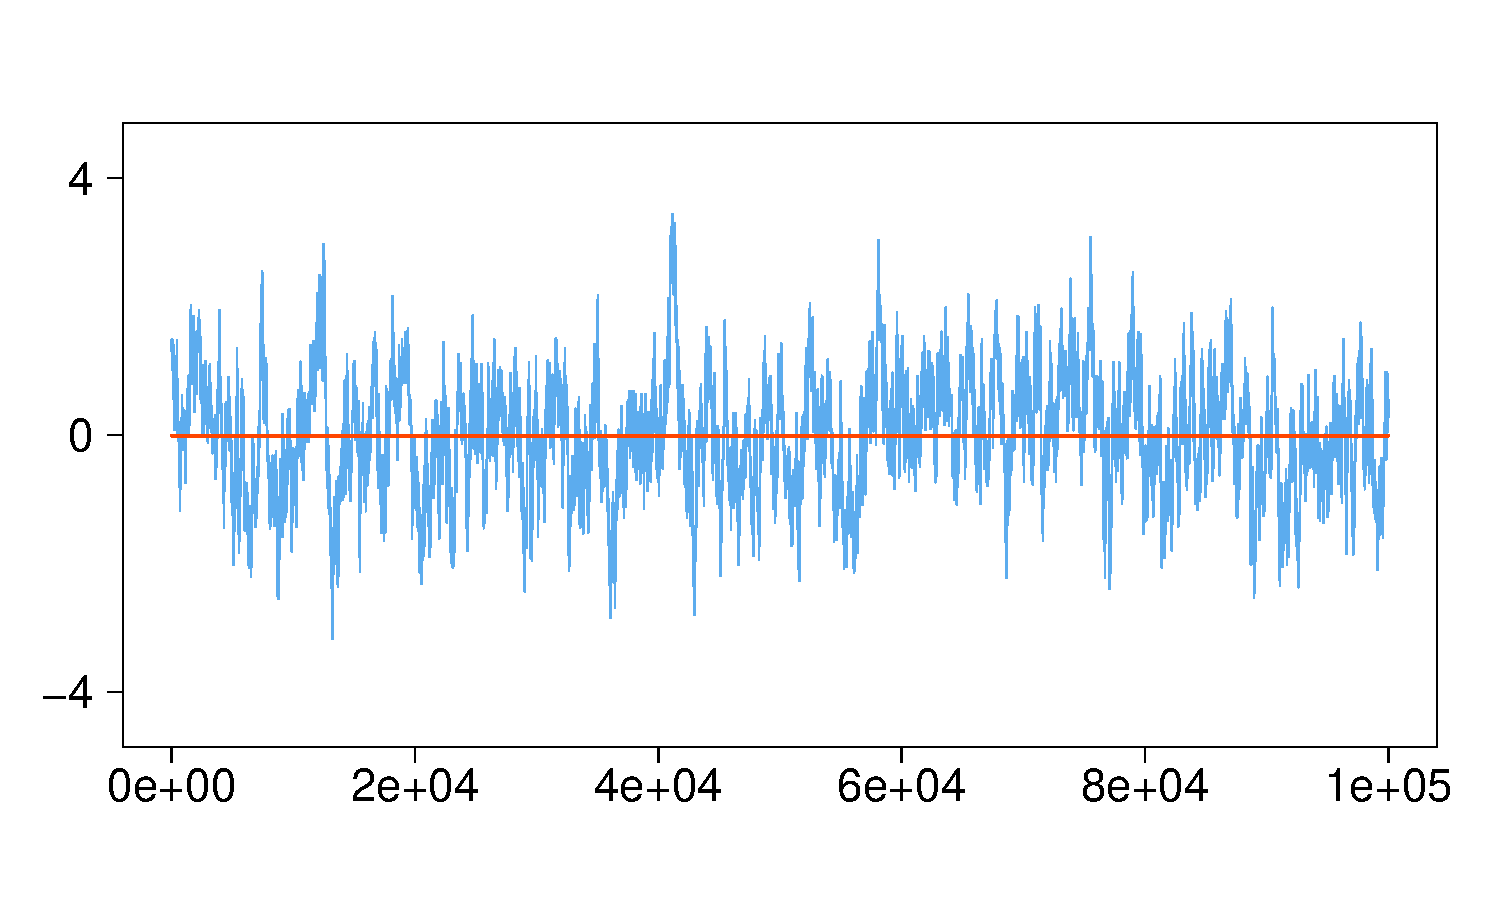
\includegraphics[width=2.3in]{tdist_smmala_traceplot.pdf}} \\
	\subfloat[AMSMMALA traceplot]{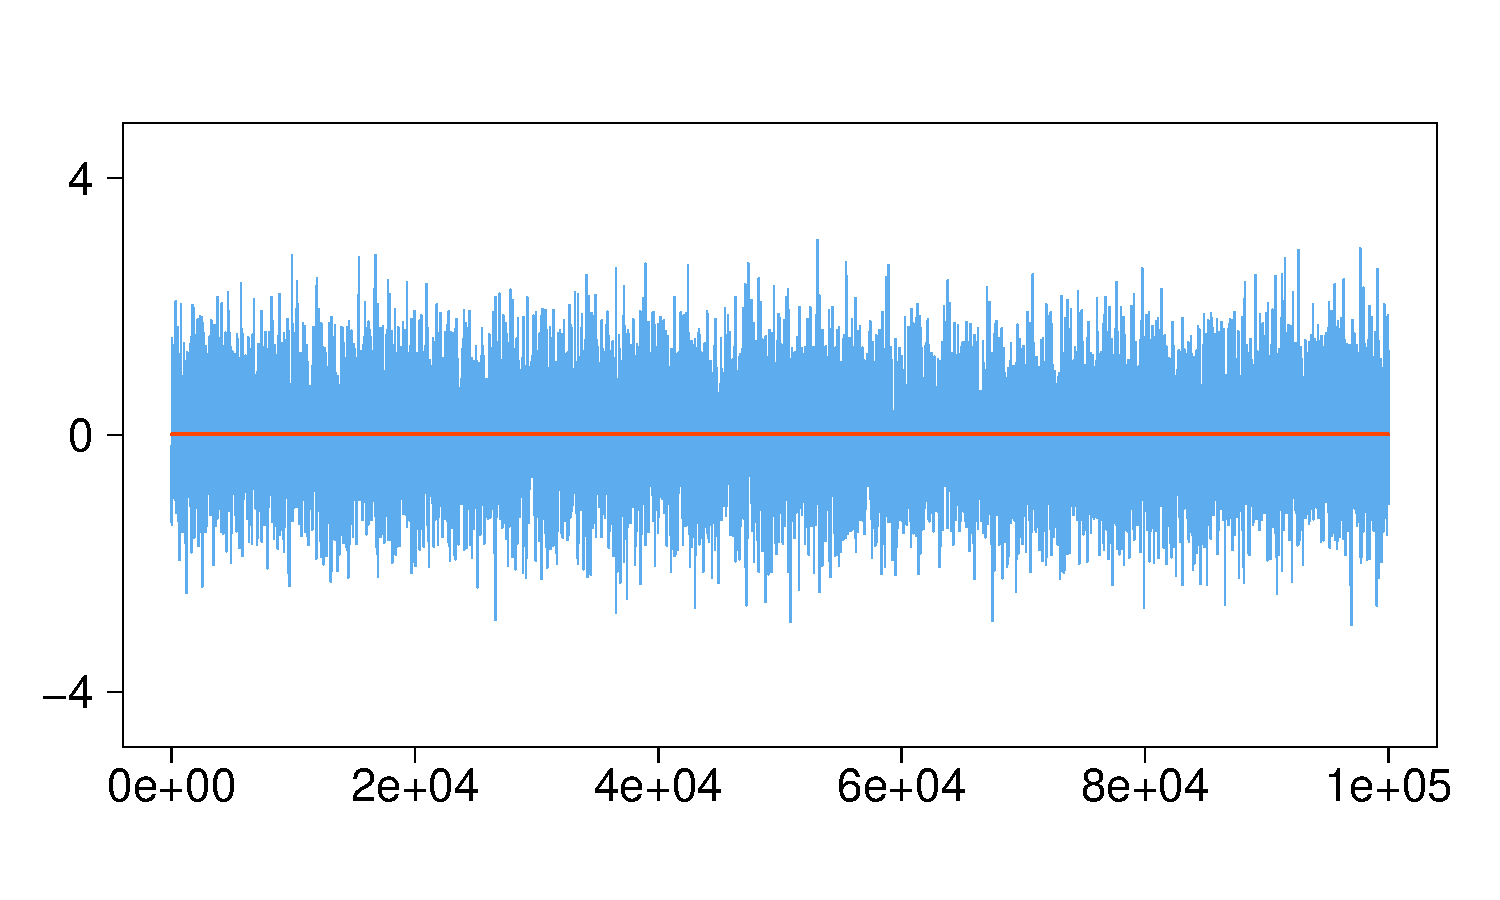
\includegraphics[width=2.3in]{tdist_amsmmala_traceplot.pdf}}
	\subfloat[ALSMMALA traceplot]{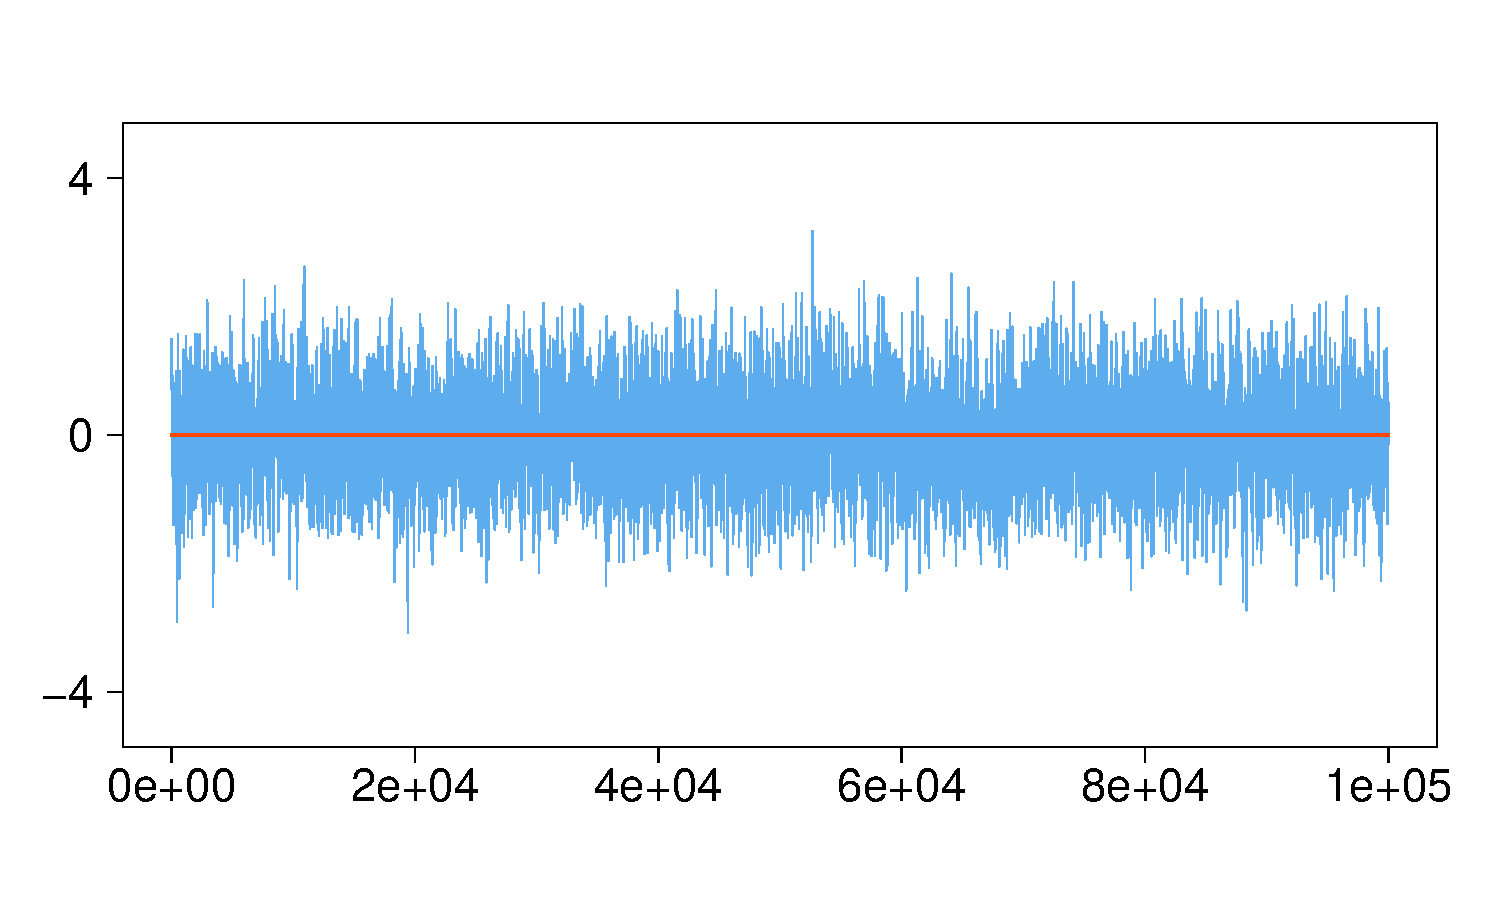
\includegraphics[width=2.3in]{tdist_alsmmala_traceplot.pdf}} \\
	\caption{t-density target - plots}
	\label{fig:t}
\end{figure}

\newpage
\section{Discussion}

% Potential for applicability in intensive applications
% It will be tried with thermodynamic integration

% Acknowledgements should go at the end, before appendices and references

\acks{We would like to acknowledge support for this project from the National Science Foundation (NSF grant IIS-9988642).}

% Manual newpage inserted to improve layout of sample file - not
% needed in general before appendices/bibliography.

\newpage

\vskip 0.2in
\bibliography{papamarkou2016}

\end{document}
